% !TEX root = ../ComputationalOTFnT.tex

\chapter{Theoretical Foundations}
\label{c-continuous}

This chapter describes the basics of optimal transport, introducing first the related notions of optimal matchings and couplings between probability vectors $(\a,\b)$, generalizing gradually this computation to transport between discrete measures $(\al,\be)$, to cover lastly the general setting of arbitrary measures. At first reading, these last nuances may be omitted and the reader can only focus on computations between probability vectors, namely histograms, which is the only requisite to implement algorithms detailed in Chapters~\ref{c-algo-basics} and~\ref{c-entropic}. More experienced readers will reach a better understanding of the problem by considering the formulation that applies to arbitrary measures, and will be able to apply it for more advanced problems (\eg in order to move positions of clouds of points, or in a statistical setting where points are sampled from continuous densities).

%%%%%%%%%%%%%%%%%%%%%%%%%%%%%%%%%%%%%%%%%%%%
\section{Histograms and Measures}

We will use interchangeably the terms histogram and probability vector for any element $\a \in \simplex_n$ that belongs to the probability simplex
\eq{
	\simplex_n \eqdef \enscond{\a \in \RR_+^n}{ \sum_{i=1}^n \a_i = 1 }.
}
A large part of this review focuses exclusively on the study of the geometry induced by optimal transport on the simplex. % A more versatile presentation takes advantage of the formalism of discrete measures, which corresponds to handling both the weights contained in a probability vector and the positions associated with the bins of the histogram (the support of the measure). % This formalism can be used implicitly to handle histograms of arbitrary size $n$ and with possibly varying positions. Lastly, the third and most technical layer of exposition deals with arbitrary measures (\ie which need not be discrete, typically continuous with respect to a base measure).


%%%%%%%%%%%%%%
\begin{rem1}{Discrete measures}
A discrete measure with weights $\a$ and locations $x_1,\dots,x_n\in\X$ reads
\eql{\label{eq-discr-meas}
	\al = \sum_{i=1}^n \a_i \de_{x_i},
}
where $\de_x$ is the Dirac at position $x$, intuitively a unit of mass which is infinitely concentrated at location $x$. Such a measure describes a probability measure if, additionally, $\a\in\simplex_n$ and more generally a positive measure if all the elements of vector $\a$ are nonnegative. To avoid degeneracy issues where locations with no mass are accounted for, we will assume when considering discrete measures that all the elements of $\a$ are positive.
\end{rem1}
%%%%%%%%%%%%%%



%%%%%%%%%%%%%%
\begin{rem2}{General measures}
A convenient feature of OT is that it can deal with measures that are either or both discrete and continuous within the same framework. To do so, one relies on the set of Radon measures $\Mm(\X)$ on the space $\X$. The formal definition of that set
requires that $\X$ is equipped with a distance, usually denoted $\dist$, because one can access a measure only by ``testing'' (integrating) it against continuous functions, denoted $f \in \Cc(\X)$.

Integration of $f \in \Cc(\X)$ against a discrete measure $\al$ computes a sum
\eq{
	\int_\X f(x) \d\al(x) = \sum_{i=1}^n \a_i f(x_i).
}
%
More general measures, for instance on $\X=\RR^\dim$ (where $\dim \in \NN^*$ is the dimension), can have a density $\d\al(x)=\density{\al}(x)\d x$ w.r.t. the Lebesgue measure, often denoted $\density{\al} = \frac{\d\al}{\d x}$, which means that
\eq{
	\foralls h \in \Cc(\RR^\dim), \quad
	\int_{\RR^\dim} h(x) \d\al(x) =  \int_{\RR^\dim} h(x) \density{\al}(x) \d x.
}
%
An arbitrary measure $\al \in \Mm(\X)$ (which need not have a density nor be a sum of Diracs) is defined by the fact that it can be integrated against any continuous function $f \in \Cc(\X)$ and obtain $\int_\X f(x) \d\al(x) \in \RR$. If $\X$ is not compact, one should also impose that $f$ has compact support or at least has $0$ limit at infinity.
%
Measures are thus in some sense ``less regular'' than functions but more regular than distributions (which are dual to smooth functions). For instance, the derivative of a Dirac is not a measure.
%
We denote $\Mm_+(\X)$ the set of all positive measures on $\X$. The set of probability measures is denoted $\Mm_+^1(\X)$, which means that any $\al \in \Mm_+^1(\X)$ is positive, and that $\al(\X)=\int_\Xx \d\al = 1$.
%
Figure~\ref{fig-measures} offers a visualization of the different classes of measures, beyond histograms, considered in this work.
\end{rem2}
%%%%%%%%%%%%%%


\begin{figure}[h!]
\centering
\begin{tabular}{@{}c@{\hspace{1mm}}c@{\hspace{1mm}}c@{\hspace{1mm}}c@{}}
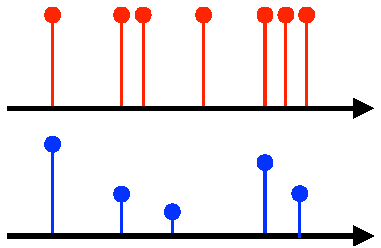
\includegraphics[width=.24\linewidth]{measures/discrete-1d.pdf}&
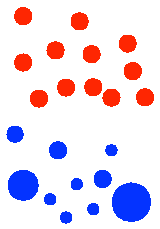
\includegraphics[width=.15\linewidth]{measures/discrete-2d}&
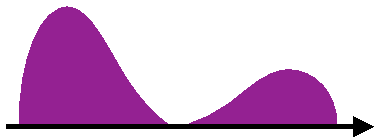
\includegraphics[width=.24\linewidth]{measures/density-1d}&
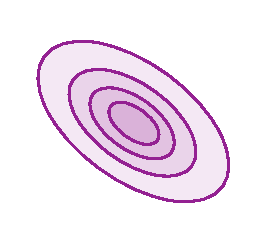
\includegraphics[width=.22\linewidth]{measures/density-2d}\\
Discrete $d=1$ & Discrete $d=2$ & Density $d=1$ & Density $d=2$
\end{tabular}
\caption{\label{fig-measures}
Schematic display of discrete distributions $\al = \sum_{i=1}^n \a_i \de_{x_i}$ (red corresponds to empirical uniform distribution $\a_i=1/n$, and blue to arbitrary distributions) and densities $\d\al(x)=\density{\al}(x)\d x$ (in purple), in both one and two dimensions. Discrete distributions in one-dimension are displayed as stem plots (with length equal to $\a_i$) and in two dimensions using point clouds (in which case their radius might be equal to $\a_i$ or, for a more visually accurate representation, their area).
}
\end{figure}





%%%%%%%%%%%%%%%%%%%%%%%%%%%%%%%%%%%%%%%%%%%%
\section{Assignment and Monge Problem}

Given a cost matrix $(\C_{i,j})_{i \in \range{n}, j \in \range{m}}$, assuming $n=m$, the optimal assignment problem seeks for a bijection $\si$ in the set $\Perm(n)$ of permutations of $n$ elements solving
\eql{\label{eq-optimal-assignment}
	\umin{\si \in \Perm(n)} \frac{1}{n}\sum_{i=1}^n \C_{i,\si(i)}.
}
One could naively evaluate the cost function above using all permutations in the set $\Perm(n)$. However, that set has size $n!$, which is gigantic even for small $n$. Consider, for instance, that such a set has more than $10^{100}$ elements~\citep{Dantzig1983} when $n$ is as small as 70. That problem can therefore be solved only if there exist efficient algorithms to optimize that cost function over the set of permutations, which is the subject of~\S\ref{s-auction}.

\begin{rem}[Uniqueness] Note that the optimal assignment problem may have several optimal solutions. Suppose, for instance, that $n=m=2$ and that the matrix $\C$ is the pairwise distance matrix between the four corners of a 2-D square of side length $1$, as represented in the left plot of Figure~\ref{fig-non-unique-matching}. In that case only two assignments exist, and they are both optimal.
\end{rem}


\begin{figure}[h!]
\centering
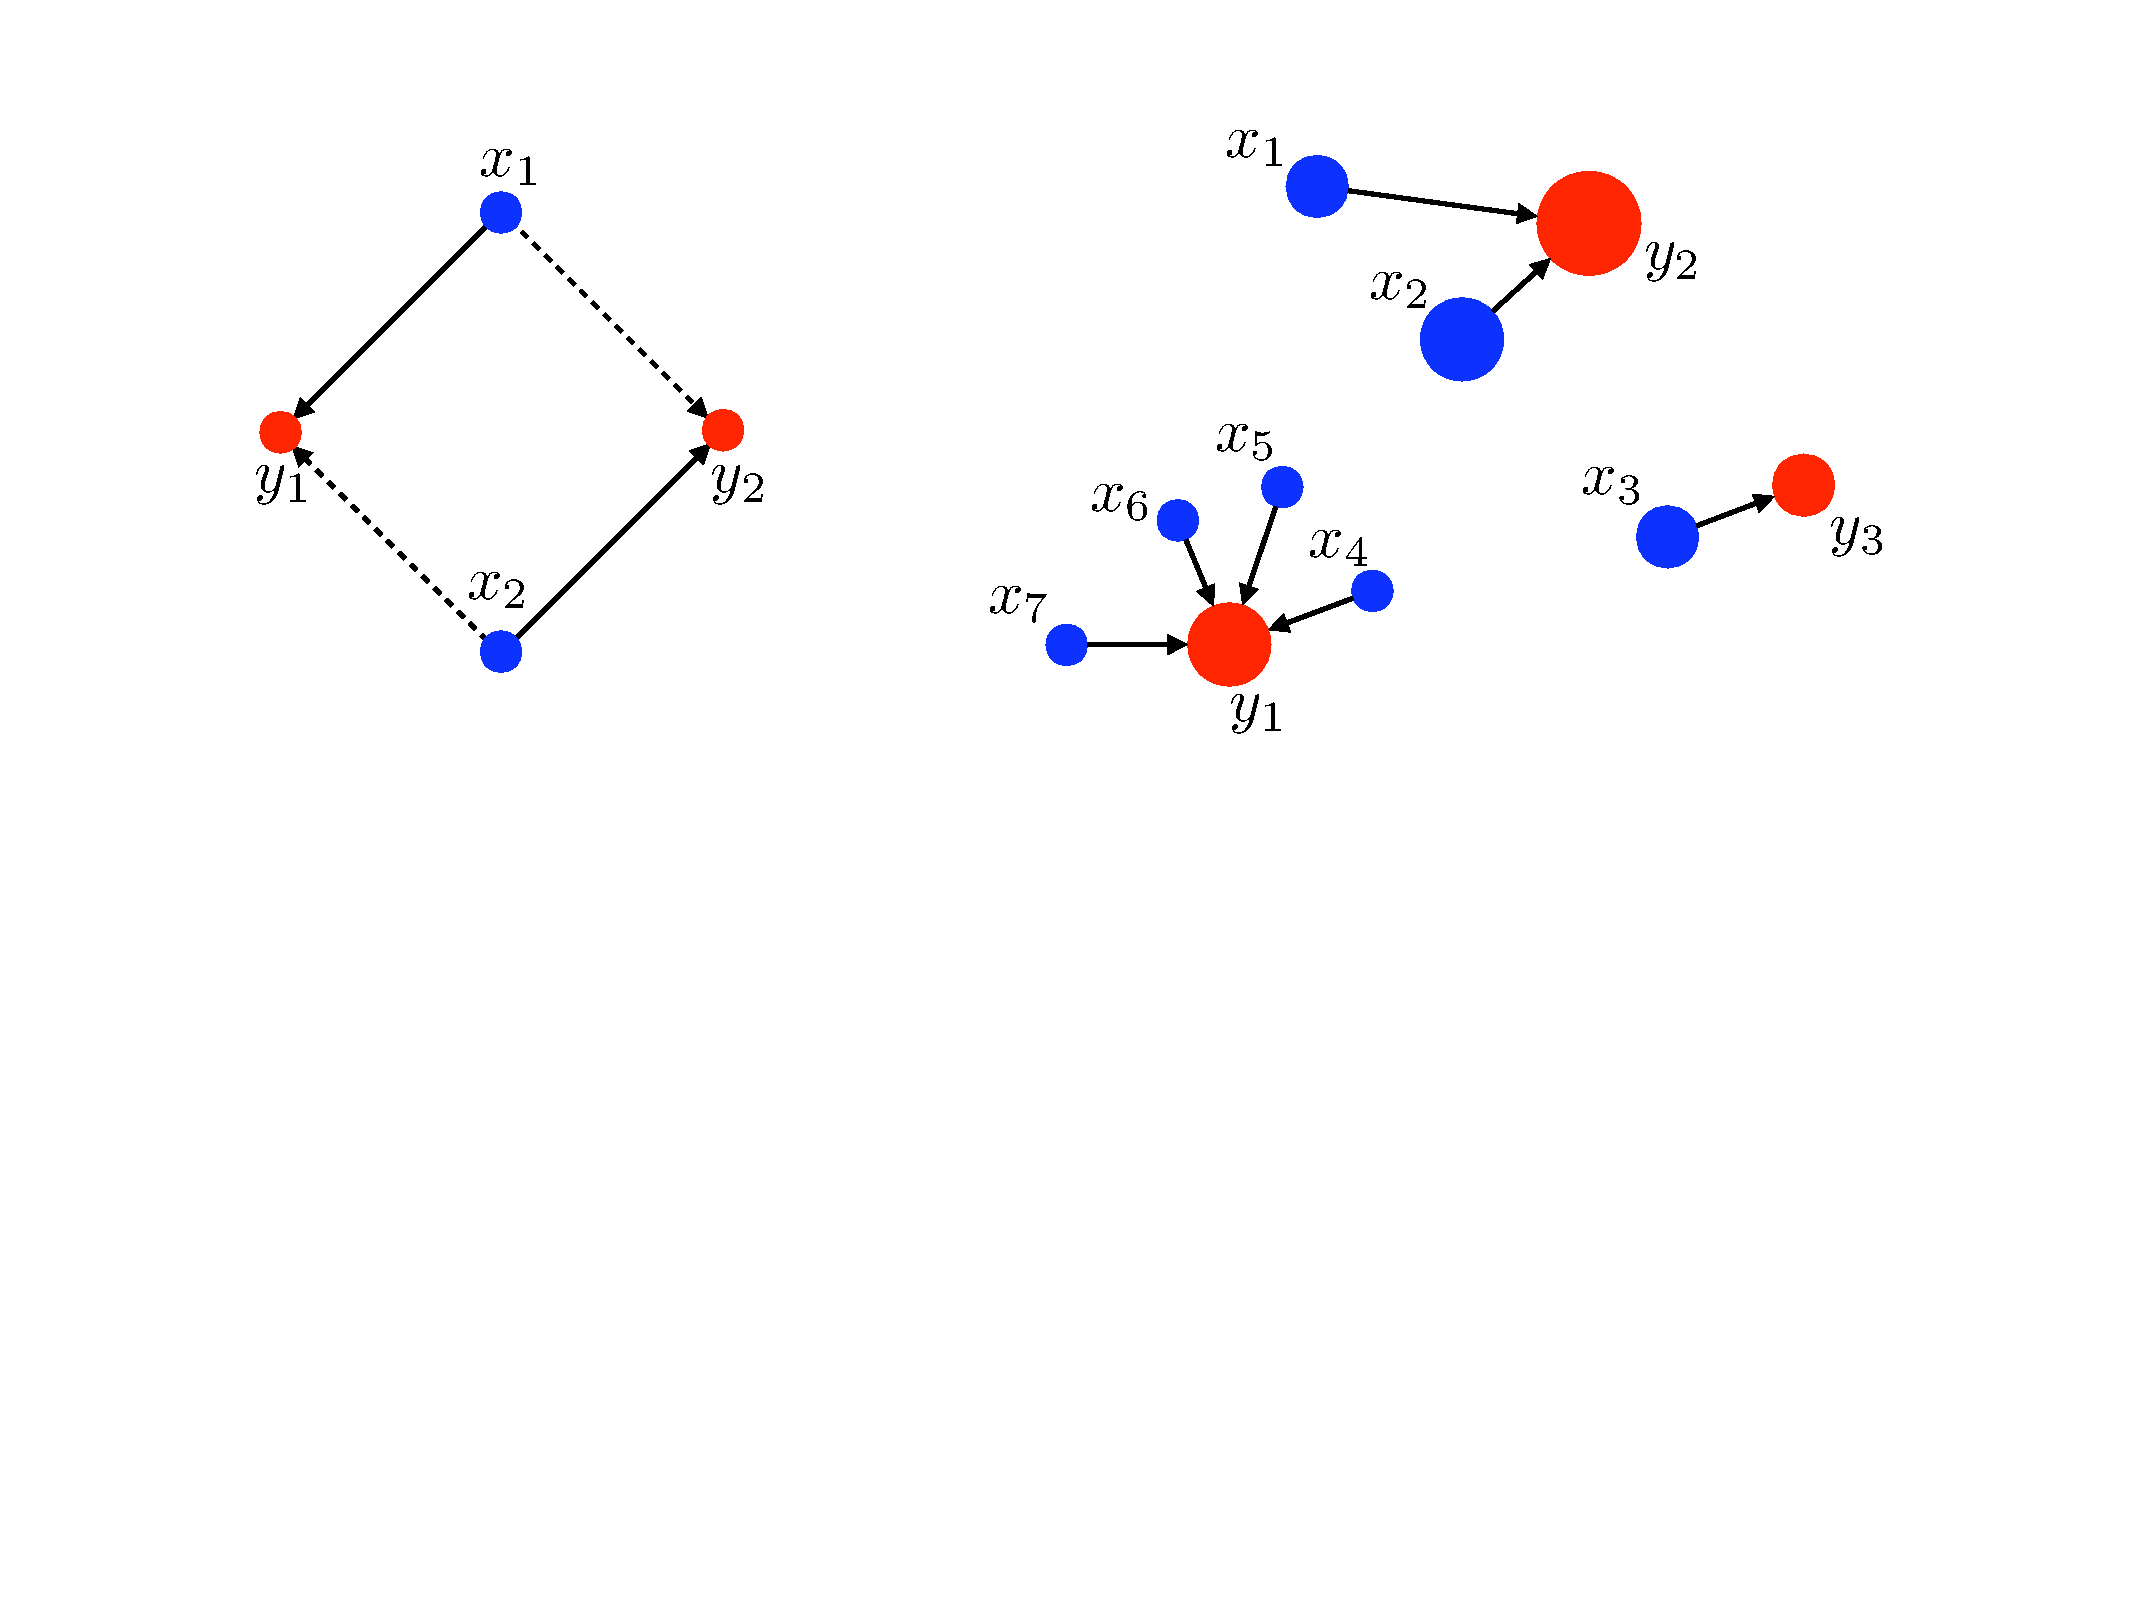
\includegraphics[width=.8\linewidth]{non-unique-optimal-matching/non-unique-optimal-matching}
\caption{\label{fig-non-unique-matching}
Left: blue dots from measure $\alpha$ and red dots from measure $\beta$ are pairwise equidistant. Hence, either matching $\sigma=(1,2)$ (full line) or $\sigma=(2,1)$ (dotted line) is optimal. Right: a Monge map can associate the blue measure $\alpha$ to the red measure $\beta$. The weights $\alpha_i$ are displayed proportionally to the area of the disk marked at each location. The mapping here is such that $T(x_1)=T(x_2)=y_2$, $T(x_3)=y_3$, whereas for $4\leq i\leq 7$ we have $T(x_i)=y_1$.
}
\end{figure}


%%%%%%%%%
\begin{rem1}{Monge problem between discrete measures}\label{rem-monge1}
For dis\-cre\-te measures
\eql{\label{eq-pair-discr}
	\al = \sum_{i=1}^n \a_i \de_{x_i}
	\qandq
	\be = \sum_{j=1}^m \b_j \de_{y_j},
}
the~\citeauthor{Monge1781} problem~\citeyearpar{Monge1781} seeks a map that associates to each point $x_i$ a single point $y_j$ and which must push the mass of $\al$ toward the mass of $\be$, namely, such a map $T:\{x_1,\dots, x_n\}\rightarrow \{y_1,\dots,y_m\}$ must verify that
\eql{\label{eq-monge-constr}
	\foralls j \in \range{m}, \quad
	\b_j = \sum_{ i : \T(x_i) = y_j } \a_i ,
}
which we write in compact form  as $\T_\sharp \al = \be$. Because all the elements of $\b$ are positive, that map is necessarily surjective.
%
This map should minimize some transportation cost, which is parameterized by a function $\c(x,y)$ defined for points $(x,y) \in \X \times \Y$,
\eql{\label{eq-monge-discr}
	\umin{\T} \enscond{ \sum_{i} \c(x_i,\T(x_i))  }{ \T_\sharp \al = \be } .
}
Such a map between discrete points can be of course encoded, assuming all $x$'s and $y$'s are distinct, using indices $\si : \range{n} \rightarrow \range{m}$ so that $j=\si(i)$, and the mass conservation is written as
\eq{
	\sum_{i \in \si^{-1}(j)} \a_i = \b_j,
}
where the inverse $\si^{-1}(j)$ is to be understood as the preimage set of $j$. In the special case when $n=m$ and all weights are uniform, that is, $\a_i=\b_j=1/n$, then the mass conservation constraint implies that $\T$ is a bijection, such that $\T(x_i)=y_{\si(i)}$, and the Monge problem is equivalent to the optimal matching problem~\eqref{eq-optimal-assignment}, where the cost matrix is
\eq{
	\C_{i,j} \eqdef \c(x_i,y_j).
}
When $n\ne m$, note that, optimality aside, Monge maps may not even exist between a discrete measure to another. This happens when their weight vectors are not compatible, which is always the case when the target measure has more points than the source measure, $n<m$. For instance, the right plot in Figure~\ref{fig-non-unique-matching} shows an (optimal) Monge map between $\al$ and $\be$, but there is no Monge map from $\be$ to $\al$.
\end{rem1}
%%%%%%%%%


%%%%%%%
\begin{rem2}{Push-forward operator}\label{rem-push-f}
For a continuous map $\T : \X \rightarrow \Y$, we define its corresponding push-forward operator $\T_\sharp : \Mm(\X) \rightarrow \Mm(\Y)$.
%
For discrete measures~\eqref{eq-discr-meas}, the push-forward operation consists simply in moving the positions of all the points in the support of the measure
\eq{
	\T_{\sharp} \al \eqdef \sum_i \a_i \de_{\T(x_i)}.
}
For more general measures, for instance, for those with a density, the notion of push-forward plays a fundamental role to describe the spatial modification (or transport) of a probability measure. The formal definition reads as follows.

\begin{defn}[Push-forward]\label{defn-pushfwd}
For $\T : \X \rightarrow \Y$, the push-forward measure $\be = \T_\sharp \al \in \Mm(\Y)$ of some $\al \in \Mm(\X)$ satisfies
\eql{\label{eq-push-fwd}
	\foralls h \in \Cc(\Y), \quad \int_\Y h(y) \d \be(y) = \int_\X h(\T(x)) \d\al(x).
	% = \int_X h(T(x)) \density{\al}(x) \d x %%%% y=T(x)   dy=|T'(x)| dx
	% = \int_Y h(y) \density{\al}(T^{-1}(y)) 1/|T'(x)| \d y
	% = \int_Y h(y) \density{\be}(y) \d y
	%  \density{\al}(T^{-1}(y)) 1/|T'(x)| = \density{\be}(y)
}
Equivalently, for any measurable set $B \subset \Y$, one has
\eql{\label{eq-equiv-pushfwd}
	\be(B) = \al( \enscond{x \in \X}{\T(x) \in B} ) = \al( T^{-1}(B) ).
}
Note that $\T_\sharp$ preserves positivity and total mass, so that if $\al \in \Mm_+^1(\X)$ then $\T_\sharp \al \in \Mm_+^1(\Y)$.
\end{defn}

Intuitively, a measurable map $T: \X\rightarrow \Y$ can be interpreted as a function moving a single point from a measurable space to another. $T_\sharp$ is an extension of $T$ that can move an entire probability measure on $\X$ toward a new probability measure on $\Y$. The operator $T_\sharp$ \emph{pushes forward} each elementary mass of a measure $\al$ on $\X$ by applying the map $T$ to obtain then an elementary mass in $\Y$.  Note that a push-forward operator $\T_\sharp : \Mm_+^1(\X) \rightarrow \Mm_+^1(\Y)$ is \emph{linear} in the sense that for two measures $\al_1,\al_2$ on $\X$, $T_\sharp(\al_1+\al_2)=T_\sharp\al_1+ T_\sharp\al_2$.
\end{rem2}
%%%%%%%

%%%%%%%
\begin{rem2}{Push-forward for multivariate densities}
Explicitly doing the change of variables in formula~\eqref{eq-push-fwd} for measures with densities $(\density{\al},\density{\be})$ on $\RR^\dim$ (assuming $\T$ is smooth and bijective) shows that a push-forward acts on densities linearly as a change of variables in the integration formula. Indeed, one has
\eql{\label{eq-pfwd-density}
	\density{\al}(x) = |\det(\T'(x))|  \density{\be}(\T(x)),
}
where $\T'(x) \in \RR^{\dim \times \dim}$ is the Jacobian matrix of $T$ (the matrix formed by taking the gradient of each coordinate of $T$).
This implies
\eq{
	|\det(\T'(x))| = \frac{ \density{\al}(x) }{ \density{\be}(\T(x)) }.
}
\end{rem2}
%%%%%%%


%%%%%%%
\begin{rem2}{Monge problem between arbitrary measures}\label{rem-monge2}
The Mon\-ge problem~\eqref{eq-monge-discr} can be extended to the case where two arbitrary probability measures $(\al,\be)$, supported on two spaces $(\X,\Y)$ can be linked through a map $\T : \X \rightarrow \Y$ that minimizes
\eql{\label{eq-monge-continuous}
	\umin{\T} \enscond{ \int_{\X} \c(x,\T(x)) \d \al(x)  }{  \T_\sharp \al = \be }.
}
The constraint $\T_\sharp \al = \be$ means that $\T$ pushes forward the mass of $\al$ to $\be$, using the push-forward operator defined in Remark~\ref{rem-push-f}
\end{rem2}
%%%%%%%


%%%%%%%
\begin{rem2}{Push-forward vs. pull-back}
The push-forward $\T_\sharp$ of measures should not be confused with the pull-back of functions $\T^\sharp : \Cc(\Y) \rightarrow \Cc(\X)$ which corresponds to ``warping'' between functions, defined as the linear map which to $g \in \Cc(\Y)$ associates $\T^\sharp g = g \circ \T$. Push-forward and pull-back are actually adjoint to one another, in the sense that
\eq{
	\foralls (\al,g) \in \Mm(\X) \times \Cc(\Y), \quad
	\int_\Y g \d( \T_\sharp\al ) = \int_\X (\T^\sharp g) \d\al.
}
Note that even if $(\al,\be)$ have densities $(\density{\al},\density{\be})$ with respect to a fixed measure (\emph{e.g.} Lebesgue on $\RR^\dim$), $\T_\sharp \al$ does not have $\T^\sharp \density{\be}$ as density, because of the presence of the Jacobian in~\eqref{eq-pfwd-density}.
%
This explains why OT should be used with caution to perform image registration, because it does not operate as an image warping method.
%
Figure~\ref{fig-push-pull} illustrates the distinction between these push-forward and pull-back operators.
\end{rem2}
%%%%%%%


\begin{figure}[h!]
\centering
\begin{tabular}{@{}c@{\hspace{5mm}}c@{}}
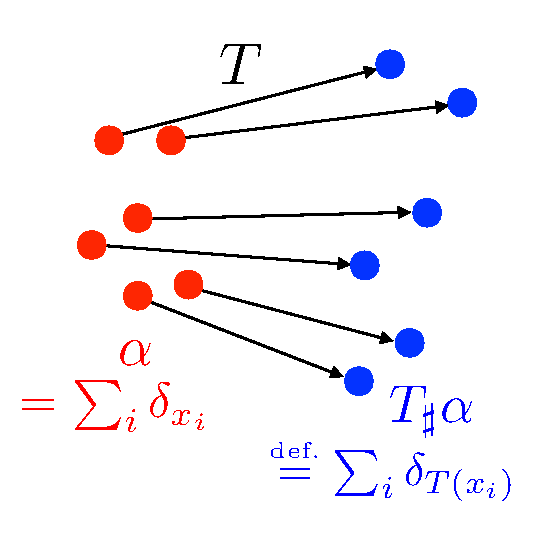
\includegraphics[width=.3\linewidth]{push-pull/push-forward}&
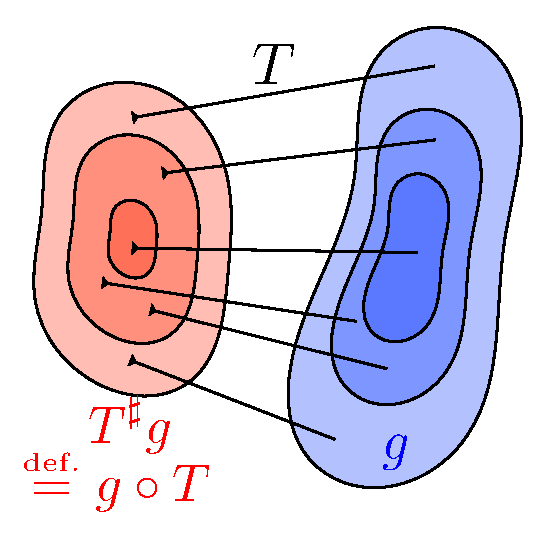
\includegraphics[width=.3\linewidth]{push-pull/pull-back}\\
Push-forward of measures & Pull-back of functions
\end{tabular}
\caption{\label{fig-push-pull}
Comparison of the push-forward operator $\T_\sharp$, which can take as an input any measure, and the pull-back operator $\T^\sharp$, which operates on functions, notaly densities.
}
\end{figure}



%%%%%%%%%%%%%%
\begin{rem2}{Measures and random variables}\label{rem-meas-random}
	Radon measures can also be viewed as representing the distributions of random variables. A random variable $X$ on $\X$ is actually a map $X : \Om \rightarrow \X$ from some abstract (often unspecified) probability space $(\Om,\PP)$, and its distribution $\al$ is the Radon measure $\al \in \Mm_+^1(\X)$ such that $\PP(X \in A) = \al(A)=\int_A \d\al(x)$.
	%
	Equivalently, it is the push-forward of $\PP$ by $X$, $\al=X_\sharp\PP$.
	%
	Applying another push-forward $\be = \T_\sharp\al$ for $\T : \X \rightarrow \Y$, following~\eqref{eq-push-fwd}, is equivalent to defining another random variable $Y=\T(X) : \om \in \Om \rightarrow \T(X(\om)) \in Y$, so that $\be$ is the distribution of $Y$.
	%
	Drawing a random sample $y$ from $Y$ is thus simply achieved by computing $y=\T(x)$, where $x$ is drawn from~$X$.
\end{rem2}
%%%%%%%%%%%%%%


%%%%%%%%%%%%%%%%%%%%%%%%%%%%%%%%%%%%%%%%%%%%
\section{Kantorovich Relaxation}\label{sec-kantorovich-relaxation}

%%%%%
%\paragraph{Limitations of the Monge Problem}

The assignment problem, and its generalization found in the Monge problem laid out in Remark~\ref{rem-monge1}, is not always relevant to studying discrete measures, such as those found in practical problems. Indeed, because the assignment problem is formulated as a permutation problem, it can only be used to compare \emph{uniform} histograms of the \emph{same} size. A direct generalization to discrete measures with nonuniform weights can be carried out using Monge's formalism of push-forward maps, but that formulation may also be degenerate in the absence of feasible solutions satisfying the mass conservation constraint~\eqref{eq-monge-constr} (see the end of Remark~\ref{rem-monge1}). Additionally, the assignment problem~\eqref{eq-monge-discr} is combinatorial, and the feasible set for the Monge problem~\eqref{eq-monge-continuous}, despite being continuously parameterized as the set consisting in all push-forward measures that satisfy the mass conservation constraint, is \emph{nonconvex}. Both are therefore difficult to solve when approached in their original formulation.

%%%%%%
% \paragraph{Kantorovich's relaxation} Redundant
The key idea of~\citet{Kantorovich42} is to relax the deterministic nature of transportation, namely the fact that a source point $x_i$ can only be assigned to another point or location $y_{\sigma_i}$ or $T(x_i)$ only. Kantorovich proposes instead that the mass at any point $x_i$ be potentially dispatched across several locations. Kantorovich moves away from the idea that mass transportation should be \emph{deterministic} to consider instead a \emph{probabilistic} transport, which allows what is commonly known now as \emph{mass splitting} from a source toward several targets. This flexibility is encoded using, in place of a permutation $\sigma$ or a map $T$, a coupling matrix $\P  \in \RR_+^{n \times m}$, where $\P_{i,j}$ describes the amount of mass flowing from bin $i$ toward bin $j$, or from the mass found at $x_i$ toward $y_j$ in the formalism of discrete measures~\eqref{eq-pair-discr}. Admissible couplings admit a far simpler characterization than Monge maps,
\eql{\label{eq-discr-couplings}
	\CouplingsD(\a,\b) \eqdef \enscond{ \P \in \RR_+^{n \times m} }{
		\P \ones_m = \a \qandq
		\transp{\P} \ones_n = \b
	},
}
where we used the following matrix-vector notation:
\eq{
	\P \ones_m = \left(\sum_j \P_{i,j}\right)_i \in \RR^n
	\qandq
	\transp{\P} \ones_n = \left(\sum_i \P_{i,j}\right)_j \in \RR^m.
}
The set of matrices $\CouplingsD(\a,\b)$ is bounded and defined by $n+m$ equality constraints, and therefore is a convex polytope (the convex hull of a finite set of matrices)~\citep[\S8.1]{brualdi2006combinatorial}.

%
Additionally, whereas the Monge formulation (as illustrated in the right plot of Figure~\ref{fig-non-unique-matching}) was intrisically asymmetric, Kantorovich's relaxed formulation is always symmetric, in the sense that a coupling $\P$ is in  $\CouplingsD(\a,\b)$ if and only if  $\transp{\P}$ is in $\CouplingsD(\b,\a)$. Kantorovich's optimal transport problem now reads
\eql{\label{eq-mk-discr}
	\MKD_{\C}(\a,\b) \eqdef
	\umin{\P \in \CouplingsD(\a,\b)}
		\dotp{\C}{\P} \eqdef \sum_{i,j} \C_{i,j} \P_{i,j}.
}
This is a linear program (see Chapter~\ref{c-algo-basics}), and as is usually the case with such programs, its optimal solutions are not necessarily unique.

\begin{rem}[Mines and factories]\label{rem-kantorovich-primal} The Kantorovich problem finds a very natural illustration in the following resource allocation problem (see also \citet{Hitchcock41}). Suppose that an operator runs $n$ warehouses and $m$ factories. Each warehouse contains a valuable raw material that is needed by the factories to run properly. More precisely, each warehouse is indexed with an integer $i$ and contains $\a_i$ units of the raw material. These raw materials must all be moved to the factories, with a prescribed quantity $\b_j$ needed at factory $j$ to function properly. To transfer resources from a warehouse $i$ to a factory $j$, the operator can use a transportation company that will charge $\C_{i,j}$ to move a single unit of the resource from location $i$ to location $j$. We assume that the transportation company has the monopoly to transport goods and applies the same linear pricing scheme to all actors of the economy: the cost of shipping $a$ units of the resource from $i$ to $j$ is equal to $a\times \C_{i,j}$.

Faced with the problem described above, the operator chooses to solve the linear program described in Equation~\eqref{eq-mk-discr} to obtain a transportation plan $\P^\star$ that quantifies for each pair $i,j$ the amount of goods $\P_{i,j}$ that must transported from warehouse $i$ to factory $j$. The operator pays on aggregate a total of $\dotp{\P^\star}{\C}$ to the transportation company to execute that plan.
\end{rem}

%%%%%%%
\paragraph{Permutation matrices as couplings.}

For a permutation $\si\in\Perm(n)$, we write $\P_{\si}$ for the corresponding permutation matrix,
	\eql{\label{eq-perm-matrices}
		\foralls (i,j) \in \range{n}^2, \quad
		(\P_{\si})_{i,j} = \choice{
			1/n \qifq j=\si_i, \\
			0 \quad\text{otherwise.}
		}
	}
One can check that in that case
\eq{\dotp{\C}{\P_{\si}}=\frac{1}{n}\sum_{i=1}^n \C_{i,\si_i},}
which shows that the assignment problem~\eqref{eq-optimal-assignment} can be recast as a Kantorovich problem~\eqref{eq-mk-discr} where the couplings $\P$ are restricted to be exactly permutation matrices:
\eq{\umin{\si \in \Perm(n)} \frac{1}{n}\sum_{i=1}^n \C_{i,\si(i)} = \umin{\si \in \Perm(n)} \dotp{\C}{\P_{\si}}.}
Next, one can easily check that the set of permutation matrices is strictly included in the \citeauthor{birkhoff} polytope $\CouplingsD(\ones_n/n,\ones_n/n)$. Indeed, for any permutation $\si$ we have $\P_{\si}\ones=\ones_n$ and $\transp{\P_{\si}}\ones=\ones_n$, whereas $\ones_n\transp{\ones_n}/n^2$ is a valid coupling but not a permutation matrix. Therefore, the minimum of $\dotp{\C}{\P}$ is necessarily smaller when considering all transportation than when considering only permutation matrices:
$$ \MKD_{\C}(\ones_n/n,\ones_n/n) \leq \umin{\si \in \Perm(n)} \dotp{\C}{\P_{\si}}.$$

The following proposition shows that these problems result in fact in the same optimum, namely that one can always find a permutation matrix that minimizes Kantorovich's problem~\eqref{eq-mk-discr} between two uniform measures $\a=\b=\ones_n/n$. The Kantorovich relaxation is therefore \emph{tight} when considered on assignment problems. %Note however that some computational algorithm, which are combinatorial in nature, are dedicated to the case of uniform histograms with the same number of points (see Chapter~\ref{c-algo-basics}).
%
Figure~\ref{fig-matching-kantorovitch} shows on the left a 2-D example of optimal matching corresponding to this special case.
%

\begin{prop}[Kantorovich for matching]\label{prop-matching-kanto}
	If $m=n$ and $\a=\b=\ones_n/n$, then there exists an optimal solution for Problem~\eqref{eq-mk-discr} $\P_{\si^\star}$, which is a permutation matrix associated to an optimal permutation $\si^\star \in \Perm(n)$ for Problem~\eqref{eq-optimal-assignment}.
\end{prop}

\begin{proof}
	\citeauthor{birkhoff}'s theorem \citeyearpar{birkhoff} states that the set of extremal points of $\CouplingsD(\ones_n/n,\ones_n/n)$ is equal to the set of permutation matrices. A fundamental theorem of linear programming \citep[Theorem 2.7]{bertsimas1997introduction} states that the minimum of a linear objective in a nonempty polyhedron, if finite, is reached at an extremal point of the polyhedron.
\end{proof}

\begin{figure}[h!]
\centering
\begin{tabular}{@{}c@{\hspace{5mm}}c@{}}
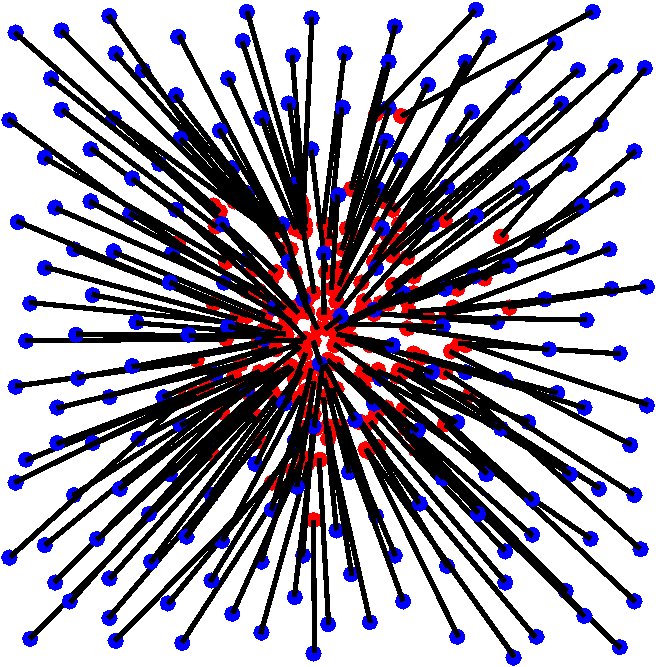
\includegraphics[width=.4\linewidth]{matching-kantorovitch/matching}&
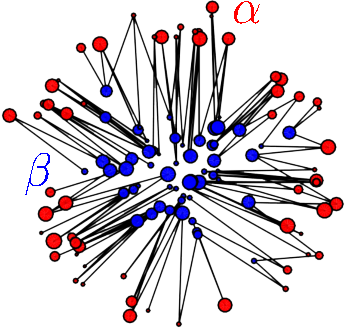
\includegraphics[width=.4\linewidth]{matching-kantorovitch/weighted}
\end{tabular}
\caption{\label{fig-matching-kantorovitch}
%
Comparison of optimal matching and generic couplings. A black segment between $x_i$ and $y_j$ indicates a nonzero element in the displayed optimal coupling $\P_{i,j}$ solving~\eqref{eq-mk-discr}.
%
Left: optimal matching, corresponding to the setting of Proposition~\ref{prop-matching-kanto} (empirical measures with the same number $n=m$ of points).
%
Right: these two weighted point clouds cannot be matched; instead a Kantorovich coupling can be used to associate two arbitrary discrete measures.
}
\end{figure}


%%%%%%%
\begin{rem1}{Kantorovich problem between discrete measures}
For discrete measures $\al,\be$ of the form~\eqref{eq-pair-discr}, we store in the matrix $\C$ all pairwise costs between points in the supports of $\al,\be$, namely $\C_{i,j} \eqdef \c(x_i,y_j)$, to define
\eql{\label{eq-kanto-discr}
	\MK_\c(\al,\be) \eqdef \MKD_{\C}(\a,\b).
}
Therefore, the Kantorovich formulation of optimal transport between discrete measures is the same as the problem between their associated probability weight vectors $\a,\b$  except that the cost matrix $\C$ depends on the support of $\al$ and $\be$. The notation $\MK_\c(\al,\be)$, however, is useful in some situations, because it makes explicit the dependency with respect to \emph{both} probability weights and supporting points, the latter being exclusively considered through the cost function $\c$.
\end{rem1}
%%%%%%%


\begin{figure}[h!]
\centering
\begin{tabular}{@{}c@{\hspace{5mm}}c@{\hspace{5mm}}c@{}}
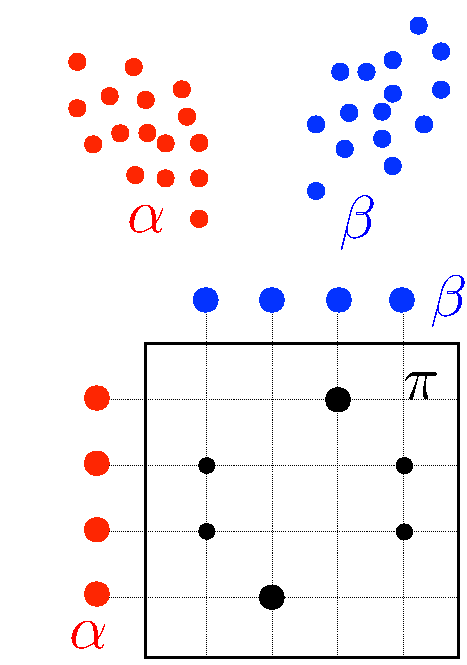
\includegraphics[width=.3\linewidth]{settings/discrete}&
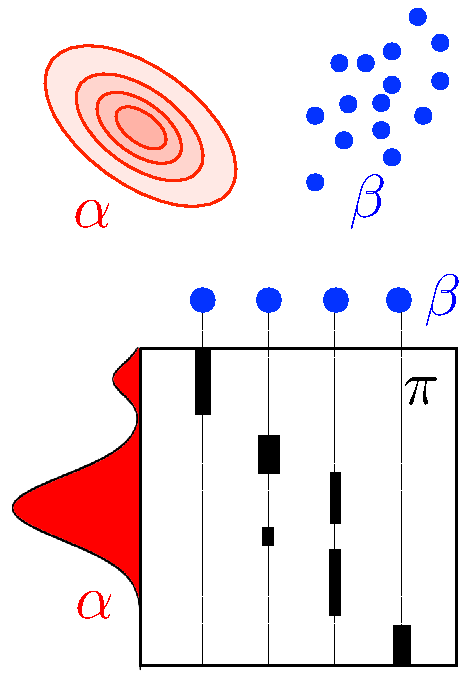
\includegraphics[width=.3\linewidth]{settings/semi-discrete}&
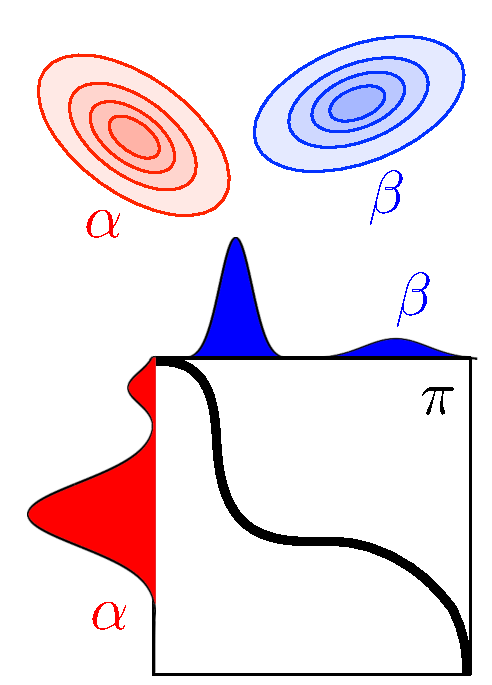
\includegraphics[width=.3\linewidth]{settings/continuous}\\
Discrete & Semidiscrete & Continuous
\end{tabular}
\caption{\label{fig-settings}
Schematic viewed of input measures $(\al,\be)$ and couplings $\Couplings(\al,\be)$ encountered in the three main scenarios for Kantorovich OT. Chapter~\ref{c-algo-semidiscr} is dedicated to the semidiscrete setup.
}
\end{figure}



%%%%%%%
\begin{rem1}{Using optimal assignments and couplings}
The op\-ti\-mal transport plan itself (either as a coupling $\P$ or a Monge map $\T$ when it exists) has found many applications in data sciences, and in particular image processing. It has, for instance, been used for contrast equalization~\citep{delon2004midway} and texture synthesis~\citet{gutierrez2017optimal}.
%
A significant part of applications of OT to imaging sciences is for image matching~\citep{zhu2007image,wang2013linear,museyko2009application,li2013novel}, image fusion~\citep{courty2016optimal}, medical imaging~\citep{wang2011optimal} and shape registration~\citep{makihara2010earth,lai2014multi,su2015optimal}, and image watermarking~\citep{mathon2014optimal}. In astrophysics, OT has been used for reconstructing the early universe~\citep{FrischNaturee}.
%
OT has also been used for music transcription~\citep{flamary2016optimal}, and finds numerous applications in economics to interpret matching data~\citep{galichon2016optimal}.
%
Lastly, let us note that the computation of transportation maps computed using OT techniques (or inspired from them) is also useful to perform sampling~\citep{reich2013nonparametric,oliver2014minimization} and Bayesian inference~\citep{kim2013efficient,el2012bayesian}.
\end{rem1}
%%%%%%%


%%%%%%%
\begin{rem2}{Kantorovich problem between arbitrary measures} De\-fi\-ni\-tion~\eqref{eq-kanto-discr} of $\MK_\c$ is extended to arbitrary measures by considering couplings $\pi \in \Mm_+^1(\X \times \Y)$ which are joint distributions over the product space. The discrete case is a special situation where one imposes this product measure to be of the form $\pi = \sum_{i,j} \P_{i,j} \de_{(x_i,y_j)}$. In the general case, the mass conservation constraint~\eqref{eq-discr-couplings} should be rewritten as a marginal constraint on joint probability distributions
\eql{\label{eq-coupling-generic}
	\Couplings(\al,\be) \eqdef
	\enscond{
		\pi \in \Mm_+^1(\X \times \Y)
	}{
		P_{\X\sharp} \pi = \al
		\qandq
		P_{\Y\sharp} \pi = \be
	}.
}
Here $P_{\X\sharp}$ and $P_{\Y\sharp}$ are the push-forwards (see Definition~\ref{defn-pushfwd}) of the projections $P_\X(x,y)=x$ and $P_\Y(x,y)=y$.
%
Figure~\ref{fig-settings} shows how these coupling constraints translate for different classes of problems (discrete measures and densities).
%
Using~\eqref{eq-equiv-pushfwd}, these marginal constraints are equivalent to imposing that $\pi(A \times \Y)=\al(A)$ and $\pi(\X \times B)=\be(B)$ for sets $A \subset \X$ and $B \subset \Y$.
%
The Kantorovich problem~\eqref{eq-mk-discr} is then generalized as
\eql{\label{eq-mk-generic}
	\MK_\c(\al,\be) \eqdef
	\umin{\pi \in \Couplings(\al,\be)}
		\int_{\X \times \Y} \c(x,y) \d\pi(x,y).
}
This is an infinite-dimensional linear program over a space of measures. If $(\X,\Y)$ are compact spaces and $c$ is continuous, then it is easy to show that it always has solutions. Indeed $\Couplings(\al,\be)$ is compact for the weak topology of measures (see Remark~\ref{dfn-weak-conv}), $\pi \mapsto \int c \d\pi$ is a continuous function for this topology and the constraint set is nonempty (for instance, $\al \otimes \be \in \Couplings(\al,\be)$).
%
Figure~\ref{fig-couplings} shows examples of discrete and continuous optimal coupling solving~\eqref{eq-mk-generic}.
%
Figure~\ref{fig-couplings-simple} shows other examples of optimal 1-D couplings, involving discrete and continuous marginals.
%
\todoK{Explain that proof of existence of minimizers (\ie the inf is a min) follows from classical reasoning in variational calculus, especially if the spaces $(\X,\Y)$ are compact (or the support of the input measure) and the cost $\c$ is continuous. Indeed, the topology to use is the weak topology of measure (Definition~\ref{dfn-weak-conv}) and then the function is continuous on a compact. }
\end{rem2}
%%%%%%%

\begin{figure}[h!]
\centering
\begin{tabular}{@{}c@{\hspace{10mm}}c@{}}
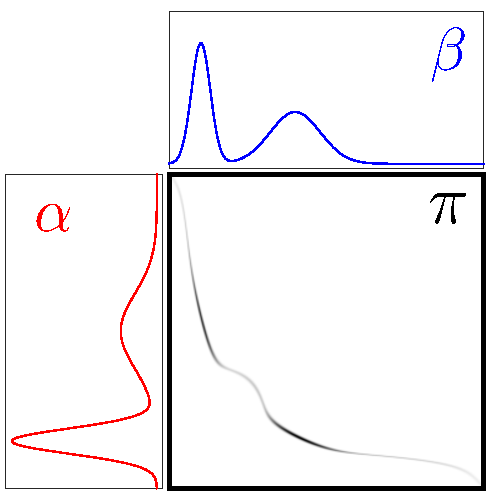
\includegraphics[width=.3\linewidth]{couplings/couplings-continuous}&
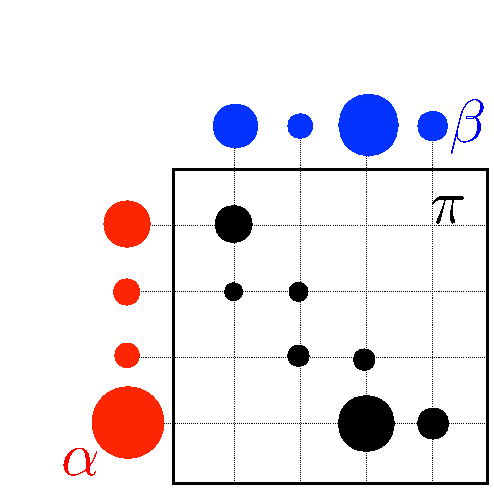
\includegraphics[width=.3\linewidth]{couplings/couplings-discr}
\end{tabular}
\caption{\label{fig-couplings}
Left: ``continuous'' coupling $\pi$ solving~\eqref{eq-coupling-generic} between two 1-D measures with density. The coupling is localized along the graph of the Monge map $(x,\T(x))$ (displayed in black).
%
Right: ``discrete'' coupling $\T$ solving~\eqref{eq-mk-discr} between two discrete measures of the form~\eqref{eq-pair-discr}. The positive entries $\T_{i,j}$  are displayed as black disks at position $(i,j)$ with radius proportional to $\T_{i,j}$.
}
\end{figure}


\begin{figure}[h!]
\centering
\begin{tabular}{@{}c@{}c@{}c@{}c@{}}
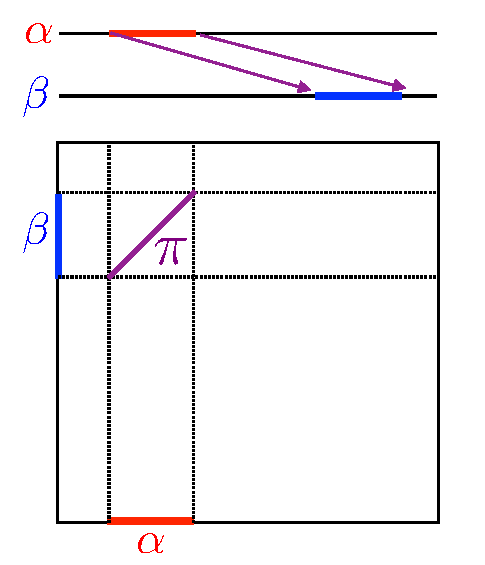
\includegraphics[width=.24\linewidth]{couplings/couplings-1}&
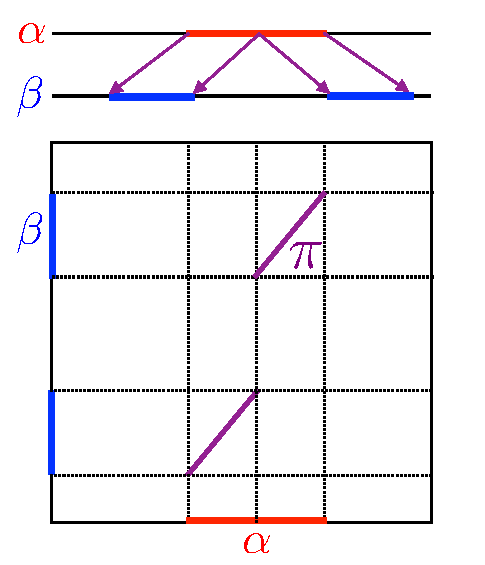
\includegraphics[width=.24\linewidth]{couplings/couplings-2}&
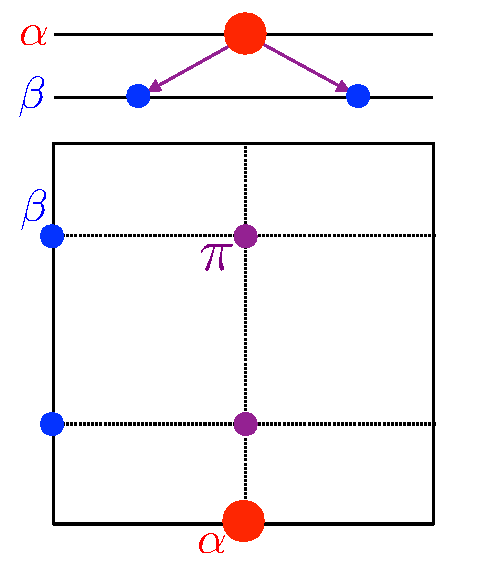
\includegraphics[width=.24\linewidth]{couplings/couplings-3}&
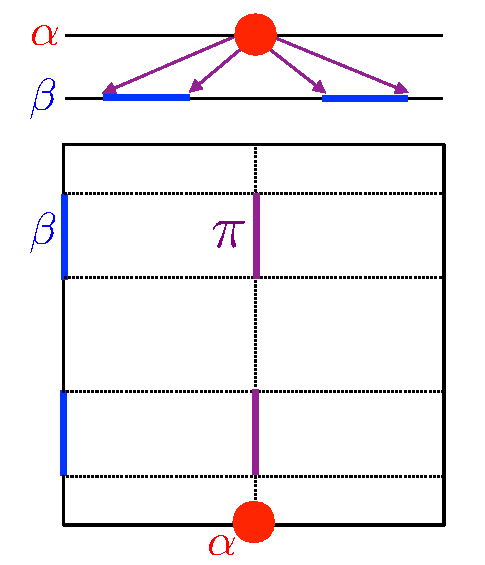
\includegraphics[width=.24\linewidth]{couplings/couplings-4}
\end{tabular}
\caption{\label{fig-couplings-simple}
Four simple examples of optimal couplings between 1-D distributions, represented as maps above (arrows) and couplings below. Inspired by~\citet{Levy2017review}.
}
\end{figure}



%%%%%%%%%%%%%%
\begin{rem2}{Probabilistic interpretation}
Kantorovich's problem can be reinterpreted through the prism of random variables, following Remark~\ref{rem-meas-random}. Indeed, Problem~\eqref{eq-mk-generic} is equivalent to
\eql{\label{eq-ot-proba-interpretation}
	\MK_\c(\al,\be) = \umin{(X,Y)} \enscond{ \EE_{(X,Y)}(c(X,Y)) }{ X \sim \al, Y \sim \be },
}
where $(X,Y)$ is a couple of random variables over $\X \times \Y$ and $X \sim \al$ (resp., $Y \sim \be$) means that the law of $X$ (resp., $Y$), represented as a measure, must be $\al$ (resp., $\be$). The law of the couple $(X,Y)$ is then $\pi \in \Couplings(\al,\be)$ over the product space $\X \times \Y$.
\end{rem2}
%%%%%%%%%%%%%%



%%%%%%%%%%%%%%%%%%%%%%%%%%%%%%%%%%%%%%%%%%%%
\section{Metric Properties of Optimal Transport}

An important feature of OT is that it defines a distance between histograms and probability measures as soon as the cost matrix satisfies certain suitable properties. Indeed, OT can be understood as a canonical way to lift a ground distance between points to a distance between histogram or measures.

We first consider the case where, using a term first introduced by~\citet{RubTomGui00}, the ``ground metric'' matrix $\C$ is fixed, representing substitution costs between bins, and shared across several histograms we would like to compare. The following proposition states that OT provides a valid distance between histograms supported on these bins.

\begin{prop}\label{prop-metric-histo}
We suppose $n=m$ and that for some $p \geq 1$, $\C=\distD^p=(\distD_{i,j}^p)_{i,j} \in \RR^{n \times n}$, where $\distD \in \RR_+^{n \times n}$ is a distance on $\range{n}$, \ie
\begin{enumerate}[label=(\roman*)]
	\item $\distD \in \RR_+^{n \times n}$ is symmetric;
	\item $\distD_{i,j}=0$ if and only if $i=j$;
	\item $\foralls (i,j,k) \in \range{n}^3, \distD_{i,k} \leq \distD_{i,j}+\distD_{j,k}$.
\end{enumerate}
Then
\eql{\label{eq-wass-p-disc}
	\WassD_p(\a,\b) \eqdef \MKD_{\distD^p}(\a,\b)^{1/p}
}
(note that $\WassD_p$ depends on $\distD$) defines the $p$-Wasserstein distance on $\Si_n$, \ie $\WassD_p$ is symmetric, positive, $\WassD_p(\a,\b)=0$ if and only if $\a = \b$, and it satisfies the triangle inequality
\eq{
	\foralls \a,\b,\VectMode{c} \in \Si_n, \quad \WassD_p(\a,\VectMode{c}) \leq \WassD_p(\a,\b) + \WassD_p(\b,\VectMode{c}).
}
\end{prop}

\begin{proof}
Symmetry and definiteness of the distance are easy to prove: since $\C = \distD^p$ has a null diagonal, $\WassD_p(\a,\a)=0$, with corresponding optimal transport matrix $\P^\star=\diag(\a)$; by the positivity of all off-diagonal elements of $\distD^p$, $\WassD_p(\a,\b)>0$ whenever $\a\ne \b$ (because in this case, an admissible coupling necessarily has a nonzero element outside the diagonal); by symmetry of $\distD^p$, $\WassD_p(\a,\b)$ is itself a symmetric function.


To prove the triangle inequality of Wasserstein distances for arbitrary measures, \citet[Theorem 7.3]{Villani03} uses the gluing lemma, which stresses the existence of couplings with a prescribed structure.
% Closed forms for such couplings exist in the discrete case which we can readily use.
In the discrete setting, the explicit constuction of this glued coupling is simple.
%
Let $\a,\b,\VectMode{c} \in\simplex_n$. Let $\P$ and $\Q$ be two optimal solutions of the transport problems between $\a$ and $\b$, and $\b$ and $\VectMode{c}$, respectively.
%
To avoid issues that may arise from null coordinates in $\b$, we define a vector $\tilde{\b}$ such that $\tilde\b_j \eqdef \b_j$ if $\b_j>0$, and $\tilde{\b}_j\eqdef 1$ otherwise, to write
\eq{
	\SS \eqdef \P \diag(1/\tilde{\b}) \Q \in \RR_+^{n \times n},
}
and notice that $\SS \in \CouplingsD(\a,\VectMode{c})$ because
\eq{
	\SS \ones_n  = \P \diag(1/\tilde{\b}) \Q \ones_n = \P (\b / \tilde{\b}) = \P \ones_{\Supp(\b)} = \a,
}
where we denoted $\ones_{\Supp(\b)}$ the vector of size $n$ with ones located at those indices $j$ where $\b_j>0$ and zero otherwise, and we use the fact that $\P \ones_{\Supp(\b)} = \P \ones = \a$ because necessarily $\P_{i,j} = 0$ for those $j$ where $\b_j=0$. Similarly one verifies that $\transp{\SS} \ones_n = \VectMode{c}$. The triangle inequality follows then from
\begin{align*}
\WassD_p(\a,\VectMode{c})&=\left(\min_{\P\in U(\a,\VectMode{c})}\dotp{\P}{\distD^p}\right)^{1/p} \leq \dotp{\SS}{\distD^p}^{1/p}\\
&= \left(\sum_{ik} \distD^p_{ik}\sum_{j} \frac{\P_{ij}\Q_{jk}}{\tilde{\b}_j}\right)^{1/p} \leq \left(\sum_{ijk} \left(\distD_{ij}+\distD_{jk}\right)^p \frac{\P_{ij}\Q_{jk}}{\tilde{\b}_j}\right)^{1/p} \\
& \leq \left(\sum_{ijk} \distD^p_{ij} \frac{\P_{ij}\Q_{jk}}{\tilde{\b}_j}\right)^{1/p} + \left(\sum_{ijk}\distD^p_{jk} \frac{\P_{ij}\Q_{jk}}{\tilde{\b}_j}\right)^{1/p}.
\end{align*}
The first inequality is due to the suboptimality of $\SS$, the second is the triangle inequality for elements in $\distD$, and the third comes from Minkowski's inequality. One thus has
\begin{align*}
\WassD_p(\a,\VectMode{c})& \leq \left(\sum_{ij} \distD^p_{ij}\P_{ij} \sum_k \frac{\Q_{jk}}{\tilde{\b}_j}\right)^{1/p} + \left(\sum_{jk} \distD^p_{jk} \Q_{jk} \sum_i \frac{\P_{ij}}{\tilde{\b}_j}\right)^{1/p}\\
&= \left(\sum_{ij} \distD^p_{ij}\P_{ij}\right)^{1/p} + \left(\sum_{jk} \distD^p_{jk} \Q_{jk}\right)^{1/p}\\
&= \WassD_p(\a,\b) +\WassD_p(\b,\c),
\end{align*}
which concludes the proof.
\end{proof}


%%%%%%%
\begin{rem}[The cases $0<p\leq 1$]
Note that if $0 < p \leq 1$, then $\distD^p$ is itself distance. This implies that while for $p\geq 1$, $\WassD_p(\a,\b)$ is a distance, in the case $p \leq 1$, it is actually $\WassD_p(\a,\b)^p$ which defines a distance on the simplex.
\end{rem}
%%%%%%%


%%%%%%%
\begin{rem1}{Applications of Wasserstein distances}
The fact that the OT distance automatically ``lifts'' a ground metric between bins to a metric between histograms on such bins makes it a method of choice for applications in computer vision and machine learning to compare histograms.
%
In these fields, a classical approach is to ``pool'' local features (for instance, image descriptors) and compute a histogram of the empirical distribution of features (a so-called bag of features) to perform retrieval, clustering or classification; see, for instance,~\citep{oliva2001modeling}.
%
Along a similar line of ideas, OT distances can be used over some lifted feature spaces to perform signal and image analysis~\citep{thorpe2017transportation}.
%
Applications to retrieval and clustering were initiated by the landmark paper~\citep{RubTomGui00}, with renewed applications following faster algorithms for threshold matrices $\C$ that fit for some applications, for example, in computer vision~\citep{pele2008linear,Pele-iccv2009}.
%
More recent applications stress the use of the earth mover's distance for bags-of-words, either to carry out dimensionality reduction~\citep{pmlr-v51-rolet16} and classify texts~\citep{kusner2015word,huang2016supervised}, or to define an alternative loss to train multiclass classifiers that output bags-of-words~\citep{FrognerNIPS}.
%
\citet{kolouri2017optimal} provides a recent overview of such applications to signal processing and machine learning.
\end{rem1}
%%%%%%%





%%%%%%%
\begin{rem1}{Wasserstein distance between measures}
Pro\-po\-si\-tion \ref{prop-metric-histo} can be generalized to deal with arbitrary measures that need not be discrete.

\begin{prop}\label{prop-metric-measure}
We assume $\X=\Y$ and that for some $p \geq 1$, $\c(x,y)=\dist(x,y)^p$, where $\dist$ is a distance on $\X$, \ie
\begin{enumerate}[label=(\roman*)]
	\item  $\dist(x,y) = \dist(y,x) \geq 0$;
	\item  $\dist(x,y)=0$ if and only if $x=y$;
	\item  $\foralls (x,y,z) \in \X^3, \dist(x,z) \leq \dist(x,y)+\dist(y,z)$.
\end{enumerate}
Then the $p$-Wasserstein distance on $\X$,
\eql{\label{eq-defn-wass-dist}
	\Wass_p(\al,\be) \eqdef \MK_{\dist^p}(\al,\be)^{1/p}
}
(note that $\Wass_p$ depends on $\dist$),  is indeed a distance, namely $\Wass_p$ is symmetric, nonnegative, $\Wass_p(\al,\be)=0$ if and only if $\al = \be$, and it satisfies the triangle inequality
\eq{
	\foralls (\al,\be,\ga) \in  \Mm_+^1(\X)^3, \quad \Wass_p(\al,\ga) \leq \Wass_p(\al,\be) + \Wass_p(\be,\ga).
}
\end{prop}
\begin{proof}
The proof follows the same approach as that for Proposition~\ref{prop-metric-histo} and relies on the existence of a coupling between $(\al,\ga)$ obtained by ``gluing'' optimal couplings between $(\al,\be)$ and $(\be,\ga)$.
\end{proof}
\end{rem1}
%%%%%%%


%%%%%%%
\begin{rem2}{Geometric intuition and weak convergence}
The Was\-ser\-stein distance $\Wass_p$ has many important properties, the most important being that it is a weak distance, \ie it allows one to compare singular distributions (for instance, discrete ones) whose supports do not overlap and to quantify the spatial shift between the supports of two distributions.
%
In particular, ``classical'' distances (or divergences) are not even defined between discrete distributions (the $L^2$ norm can only be applied to continuous measures with a density with respect to a base measure, and the discrete $\ell^2$ norm requires that positions $(x_i,y_j)$ take values in a predetermined discrete set to work properly). In sharp contrast, one has that for any $p> 0$, $\Wass_p^p(\de_x,\de_y) = \dist(x,y)$. Indeed, it suffices to notice that $\Couplings(\de_x,\de_y)=\{ \delta_{x,y}\}$ and therefore the Kantorovich problem having only one feasible solution, $\Wass_p^p(\de_x,\de_y)$ is necessarily $(\dist(x,y)^p)^{1/p}=\dist(x,y)$. This shows that $\Wass_p(\de_x,\de_y) \rightarrow 0$ if $x \rightarrow y$.
%
This property corresponds to the fact that $\Wass_p$ is a way to quantify the weak convergence, as we now define.

\begin{defn}[Weak convergence]\label{dfn-weak-conv}
	On a compact domain $\Xx$, $(\al_k)_k$ converges weakly to $\al$ in $\Mm_+^1(\Xx)$ (denoted $\al_k \rightharpoonup \al$) if and only if for any continuous function $g \in \Cc(\Xx)$, $\int_\Xx g \d\al_k \rightarrow \int_\Xx g \d\al$.
	%
	One needs to add additional decay conditions on $g$ on noncompact domains.
	%
	This notion of weak convergence corresponds to the convergence in the law of random vectors.
\end{defn}

This convergence can be shown to be equivalent to $\Wass_p(\al_k,\al) \rightarrow 0$~\citep[Theorem 6.8]{Villani09} (together with a convergence of the moments up to order $p$ for unbounded metric spaces).
\end{rem2}
%%%%%%%


%%%%%%%%%%%%%%
\begin{rem1}{Translations}
A nice feature of the Wasserstein distance over a Euclidean space $\X=\RR^\dim$ for the ground cost $c(x,y)=\norm{x-y}^2$ is that one can factor out translations; indeed, denoting $T_{\tau} : x \mapsto x-\tau$ the translation operator, one has
\eq{
	\Wass_2(T_{\tau\sharp} \al,T_{\tau'\sharp} \be)^2  =
	\Wass_2(\al,\be)^2 - 2\dotp{\tau-\tau'}{ \mean_{\al}-\mean_{\be} } + \norm{\tau-\tau'}^2,
}
\todoK{Check this!}
where $\mean_{\al} \eqdef \int_\X x \d\al(x) \in \RR^\dim$ is the mean of $\al$.
%
In particular, this implies the nice decomposition of the distance as
\eq{
	\Wass_2(\al,\be)^2  = \Wass_2(\tilde\al,\tilde{\be})^2  + \norm{\mean_{\al}-\mean_{\be}}^2,
}
where $(\tilde\al,\tilde{\be})$ are the ``centered'' zero mean measures $\tilde\al=T_{\mean_{\al}\sharp}\al$.
\end{rem1}
%%%%%%%%%%%%%%
\pagebreak
%%%%%%%
\begin{rem1}{The case $p = +\infty$}\label{rem-p-inf}
Informally, the limit of $\Wass_p^p$ as $p \rightarrow +\infty$ is
\eql{\label{eq-wass-infty}
	\Wass_{\infty}(\al,\be) \eqdef
	\umin{\pi \in \Couplings(\al,\be)}
		\usup{(x,y) \in \Supp(\pi)} d(x,y),
}
where the sup should be understood as the essential supremum according to the measure $\pi$ on $\X^2$.
%
In contrast to the cases $p<+\infty$, this is a nonconvex optimization problem, which is difficult to solve numerically and to study theoretically. The $\Wass_{\infty}$ distance is related to the Hausdorff distance between the supports of $(\al,\be)$; see \S~\ref{sec-hausdorff}. We refer to~\citep{champion2008wasserstein} for details.
\end{rem1}
%%%%%%%



%%%%%%%%%%%%%%%%%%%%%%%%%%%%%%%%%%%%%%%%%%%%
\section{Dual Problem}

The Kantorovich problem~\eqref{eq-mk-discr} is a constrained convex minimization problem, and as such, it can be naturally paired with a so-called dual problem, which is a constrained concave maximization problem. The following fundamental proposition explains the relationship between the primal and dual problems.

\begin{prop}\label{prop-duality-discr}
The Kantorovich problem~\eqref{eq-mk-discr} admits the dual
\eql{\label{eq-dual}
	\MKD_\C(\a,\b) =
	\umax{(\fD,\gD) \in \PotentialsD(\C)} \dotp{\fD}{\a} + \dotp{\gD}{\b},
}
where the set of admissible dual variables is
\eql{\label{eq-feasible-potential}
	\PotentialsD(\C) \eqdef \enscond{
		(\fD,\gD) \in \RR^n \times \RR^m
	}{ \foralls (i,j) \in \range{n} \times \range{m}, \fD \oplus \gD \leq \C }.
}
Such dual variables are often referred to as ``Kantorovich potentials.''
\end{prop}

\begin{proof}
This result is a direct consequence of the more general result on the strong duality for linear programs~\citep[p. 148, Theo. 4.4]{bertsimas1997introduction}. The easier part of the proof, namely, establishing that the right-hand side of Equation~\eqref{eq-dual} is a lower bound of $\MKD_\C(\a,\b)$, is discussed in Remark~\ref{rem-duality} in the next section.
%
For the sake of completeness, let us derive our result using Lagrangian duality. The Lagangian associated to~\eqref{eq-mk-discr} reads
\eql{\label{eq-mk-lagr}
	\umin{\P \geq 0} \umax{ (\fD,\gD) \in \RR^n \times \RR^m }
		\dotp{\C}{\P} + \dotp{\a - \P\ones_m}{\fD} + \dotp{\b - \transp{\P} \ones_n}{\gD}.
}
We exchange the min and the max above, which is always possible when considering linear programs (in finite dimension)\todoK{donner une ref}, to obtain
\eq{
	\umax{ (\fD,\gD) \in \RR^n \times \RR^m }
	\dotp{\a}{\fD} + \dotp{\b}{\gD}
	+ \umin{\P \geq 0}
		\dotp{\C - \fD\transp{\ones_m} - \ones_n \transp{\gD}}{\P}.
}
We conclude by remarking that
\eq{
	\umin{\P \geq 0} \dotp{\Q}{\P} =
	\choice{
		0 \qifq \Q \geq 0,\\
		-\infty \quad \text{otherwise}
	}
}
so that the constraint reads $\C - \fD\transp{\ones_m} - \ones_n \transp{\gD} = \C-\fD\oplus \gD \geq 0$.
\end{proof}

The primal-dual optimality relation for the Lagrangian~\eqref{eq-mk-lagr} allows us to locate the support of the optimal transport plan (see also~\S\ref{s-complementary})
\eql{\label{eq-mk-pd-rel}
\{(i,j) \in \range{n} \times \range{m} : \P_{i,j}>0\} \subset \enscond{(i,j) \in \range{n} \times \range{m}}{ \fD_i+\gD_j=\C_{i,j} }.
}


\begin{rem}\label{rem-kantorovich-dual}
Following the interpretation given to the Kantorovich problem in Remark~\ref{rem-kantorovich-primal}, we follow with an intuitive presentation of the dual. Recall that in that setup, an operator wishes to move at the least possible cost an overall amount of resources from warehouses to factories. The operator can do so by solving~\eqref{eq-mk-discr}, follow the instructions set out in $\P^\star$, and pay $\dotp{\P^\star}{\C}$ to the transportation company.

\emph{Outsourcing logistics.} Suppose that the operator does not have the computational means to solve the linear program~\eqref{eq-mk-discr}. He decides instead to outsource that task to a vendor. The vendor chooses a pricing scheme with the following structure: the vendor splits the logistic task into that of collecting and then delivering the goods and will apply a collection price $\fD_i$ to collect a unit of resource at each warehouse $i$ (no matter where that unit is sent to) and a price $\gD_j$ to deliver a unit of resource to factory $j$ (no matter from which warehouse that unit comes from). On aggregate, since there are exactly $\a_i$ units at warehouse $i$ and $\b_j$ needed at factory $j$, the vendor asks as a consequence of that pricing scheme a price of $\dotp{\fD}{\a}+\dotp{\gD}{\b}$ to solve the operator's logistic problem.

\emph{Setting prices.} Note that the pricing system used by the vendor allows quite naturally for arbitrarily negative prices. Indeed, if the vendor applies a price vector $\fD$ for warehouses and a price vector $\gD$ for factories, then the total bill will not be changed by simultaneously decreasing all entries in $\fD$ by an arbitrary number and increasing all entries of $\gD$ by that same number, since the total amount of resources in all warehouses is equal to those that have to be delivered to the factories. In other words, the vendor can give the illusion of giving an extremely good deal to the operator by paying him to collect some of his goods, but compensate that loss by simply charging him more for delivering them. Knowing this, the vendor, wishing to charge as much as she can for that service, sets vectors $\fD$ and $\gD$ to be as high as possible.

\emph{Checking prices.} In the absence of another competing vendor, the operator must therefore think of a quick way to check that the vendor's prices are reasonable. A possible way to do so would be for the operator to compute the price $\MKD_{\C}(\a,\b)$ of the most efficient plan by solving problem~\eqref{eq-mk-discr} and check if the vendor's offer is at the very least no larger than that amount. However, recall that the operator cannot afford such a lengthy computation in the first place. Luckily, there is a far more efficient way for the operator to check whether the vendor has a competitive offer. Recall that $\fD_i$ is the price charged by the vendor for picking a unit at $i$ and $\gD_j$ to deliver one at $j$. Therefore, the vendor's pricing scheme implies that transferring one unit of the resource from $i$ to $j$ costs exactly $\fD_i+\gD_j$. Yet, the operator also knows that the cost of shipping one unit from $i$ to $j$ as priced by the transporting company is $\C_{i,j}$. Therefore, if for any pair $i,j$ the aggregate price $\fD_i+\gD_j$ is strictly larger that $\C_{i,j}$, the vendor is charging more than the fair price charged by the transportation company for that task, and the operator should refuse the vendor's offer.


\begin{figure}[h!]
\centering
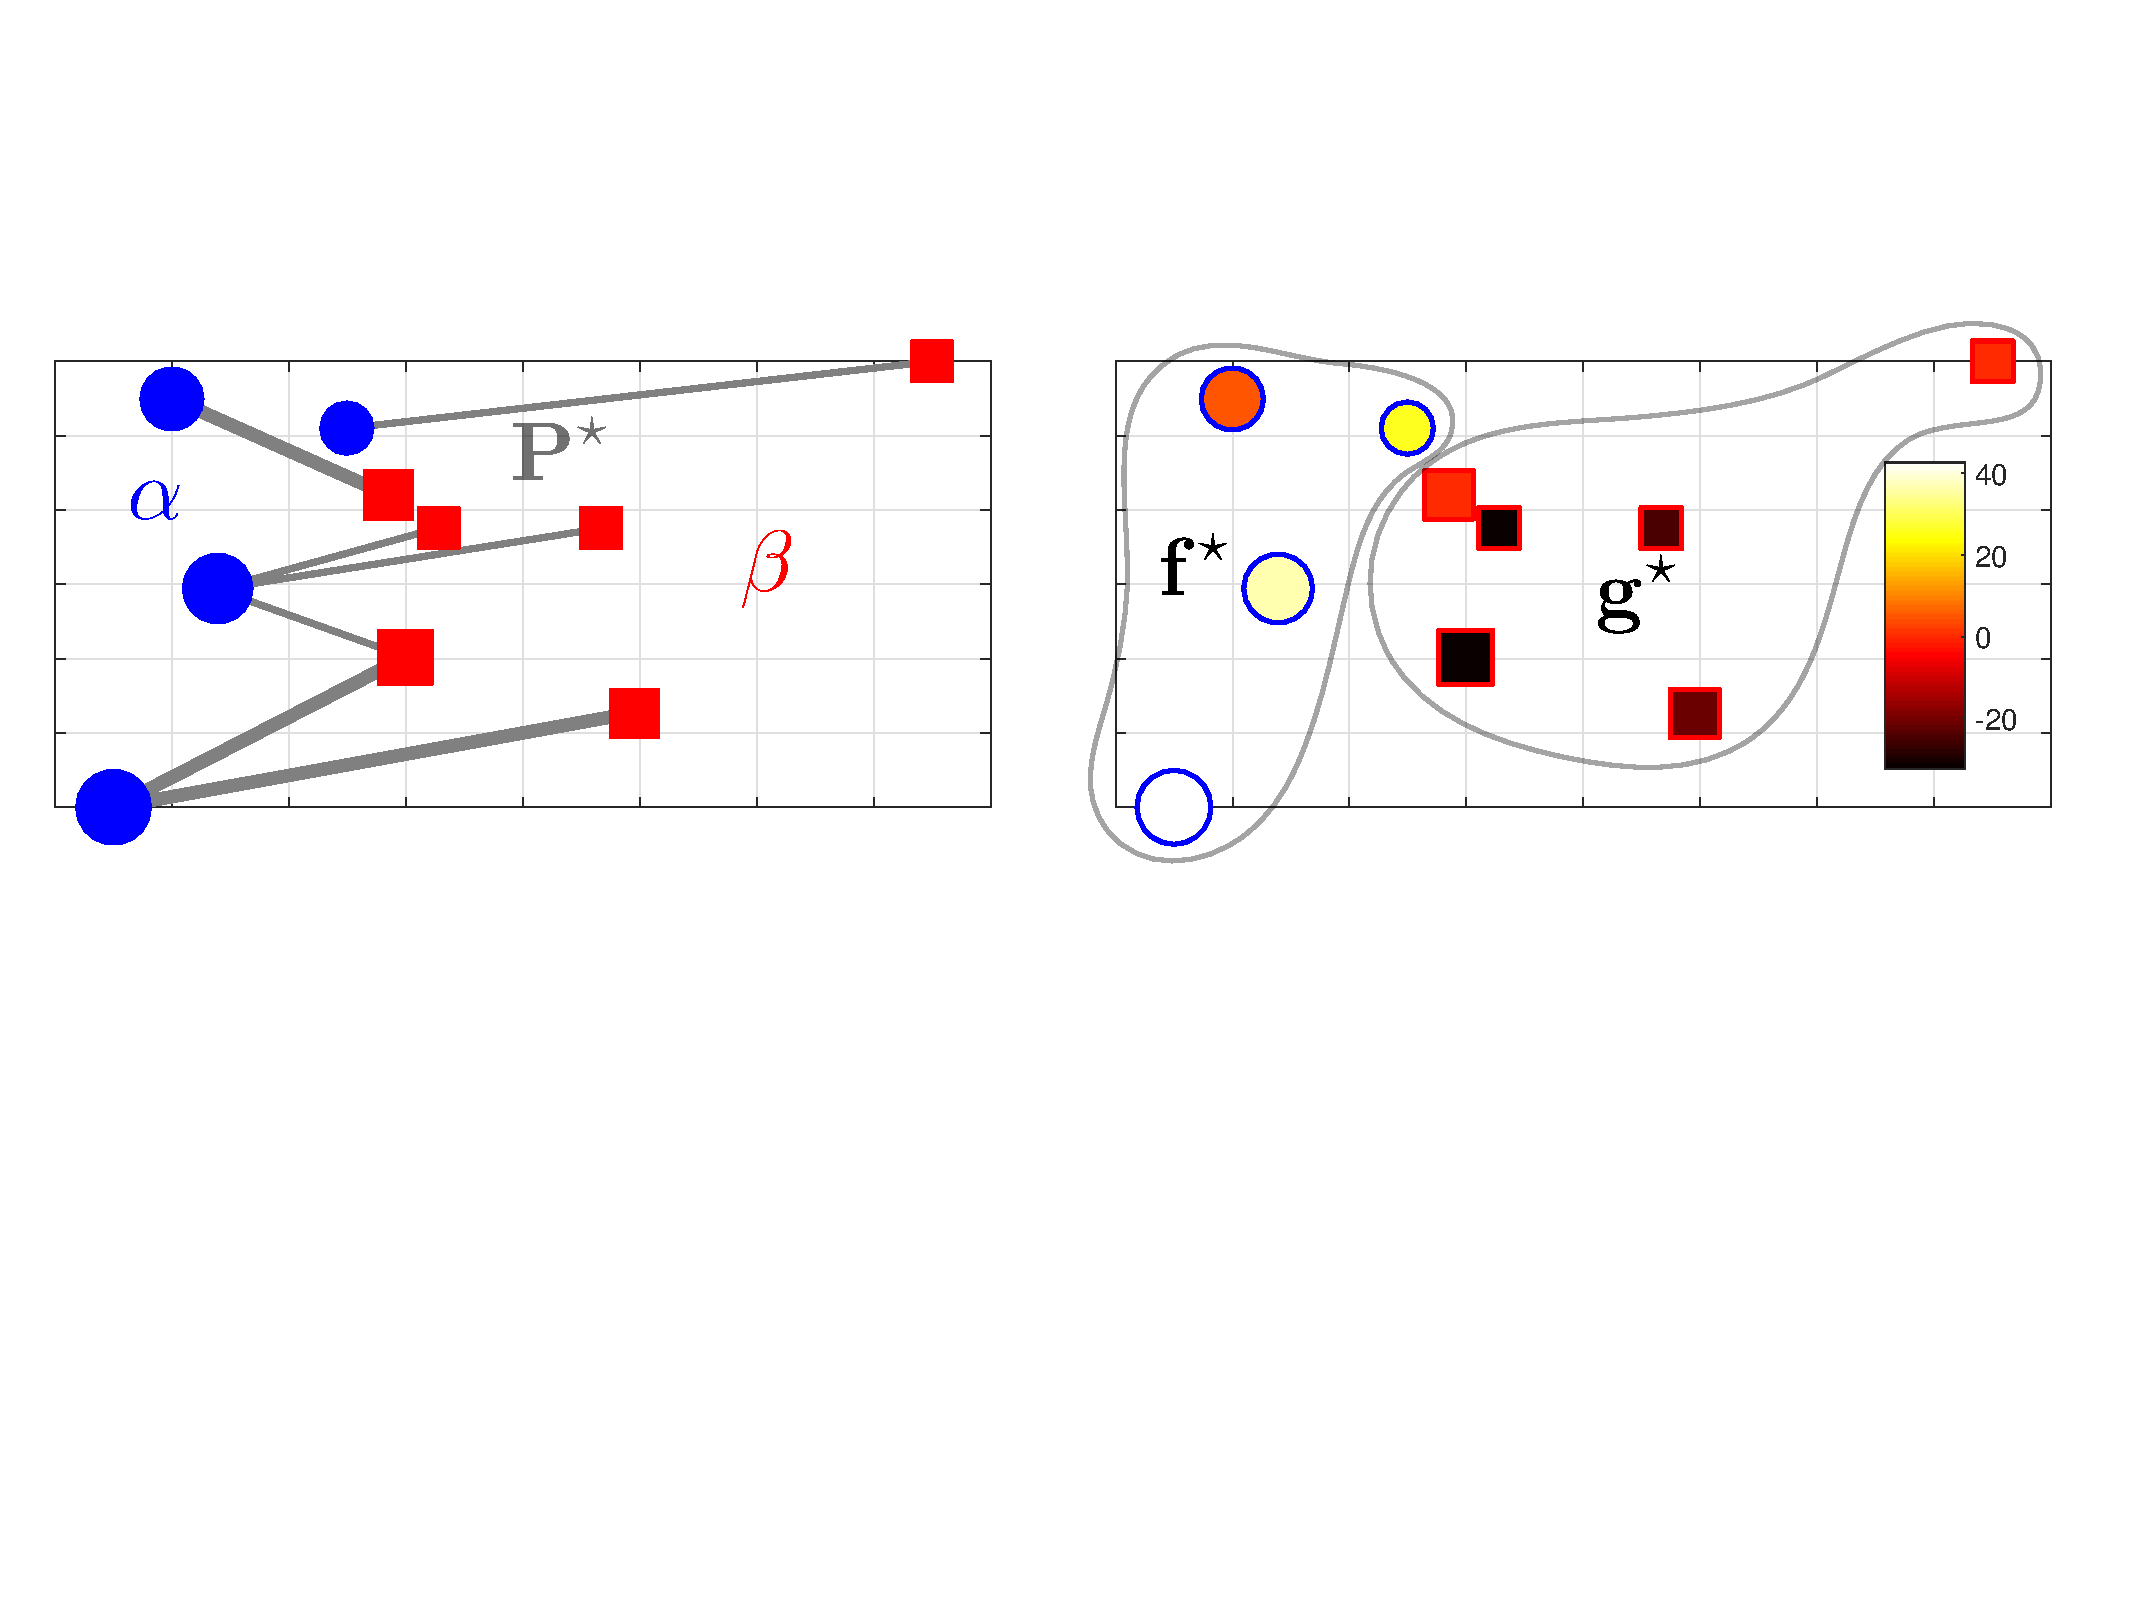
\includegraphics[width=\linewidth]{dual-solutions-overlay/dual_sols_final}
\caption{\label{dual-solutions-overlay}
Consider in the left plot the optimal transport problem between two discrete measures $\al$ and $\be$, represented respectively by blue dots and red squares. The area of these markers is proportional to the weight at each location. That plot also displays the optimal transport $\P^\star$ using a quadratic Euclidean cost. The corresponding dual (Kantorovich) potentials $\fD^\star$ and $\gD^\star$ that correspond to that configuration are also displayed on the right plot. Since there is a ``price'' $\fD_i^\star$ for each point in $\alpha$ (and conversely for $\gD$ and $\beta$), the color at that point represents the obtained value using the color map on the right. These potentials can be interpreted as relative prices in the sense that they indicate the individual cost, under the best possible transport scheme, to move a mass away at each location in $\al$, or on the contrary to send a mass toward any point in $\be$. The optimal transport cost is therefore equal to the sum of the squared lengths of all the arcs on the left weighted by their thickness or, alternatively, using the dual formulation, to the sum of the values (encoded with colors) multiplied by the area of each marker on the right plot.}
\end{figure}


\emph{Optimal prices as a dual problem.} It is therefore in the interest of the operator to check that for all pairs $i,j$ the prices offered by the vendor verify $\fD_i+\gD_j \leq \C_{i,j}$. Suppose that the operator does check that the vendor has provided price vectors that do comply with these $n\times m$ inequalities. Can he conclude that the vendor's proposal is attractive? Doing a quick back of the hand calculation, the operator does indeed conclude that it is in his interest to accept that offer. Indeed, since any of his transportation plans $\P$ would have a cost
$\dotp{\P}{\C}=\sum_{i,j} \P_{i,j}\C_{i,j}$, the operator can conclude by applying these $n\times m$ inequalities that for any transport plan $\P$ (including the optimal one $\P^\star$), the marginal constraints imply
\eq{\begin{aligned}
	\sum_{i,j} \P_{i,j}\C_{i,j} &\geq \sum_{i,j} \P_{i,j} \left(\fD_{i} + \gD_j\right) = \left(\sum_{i} \fD_{i} \sum_{j} \P_{i,j}\right) + \left(\sum_{j} \gD_{j} \sum_{i} \P_{i,j}\right)\\ 	& =\dotp{\fD}{\a}+\dotp{\gD}{\b},
\end{aligned}}
and therefore observe that \emph{any} attempt at doing the job by himself would necessarily be more expensive than the vendor's price.

Knowing this, the vendor must therefore find a set of prices $\fD,\gD$ that maximize $\dotp{\fD}{\a}+\dotp{\gD}{\b}$ but that must satisfy at the very least for all $i,j$ the basic inequality that $\fD_i+\gD_j\leq \C_{i,j}$ for his offer to be accepted, which results in Problem~\eqref{eq-dual}. One can show, as we do later in~\S\ref{s-kantorovich}, that the best price obtained by the vendor is in fact exactly equal to the best possible cost the operator would obtain by computing $\MKD_{\C}(\a,\b)$.

Figure~\ref{dual-solutions-overlay} illustrates the primal and dual solutions resulting from the same transport problem. On the left, blue dots represent warehouses and red dots stand for factories; the areas of these dots stand for the probability weights $\a,\b$, links between them represent an optimal transport, and their width is proportional to transfered amounts. Optimal prices obtained by the vendor as a result of optimizing Problem~\eqref{eq-dual} are shown on the right. Prices have been chosen so that their mean is equal to 0. The highest relative prices come from collecting goods at an isolated warehouse on the lower left of the figure, and delivering goods at the factory located in the upper right area.
\end{rem}



%%%%%%%
\begin{rem2}{Dual problem between arbitrary measures}
	To extend this primal-dual construction to arbitrary measures, it is important to realize that measures are naturally paired in duality with continuous functions (a measure can be accessed only through integration against continuous functions). The duality is formalized in the following proposition, which boils down to Proposition~\ref{prop-duality-discr} when dealing with discrete measures.

	\begin{prop}
	One has
	\eql{\label{eq-dual-generic}
		\MK_\c(\al,\be) =
		\usup{(\f,\g) \in \Potentials(\c)}
			\int_\X \f(x) \d\al(x) + \int_\Y \g(y) \d\be(y),
	}
	where the set of admissible dual potentials is
	\eql{\label{eq-dfn-pot-dual}
		\Potentials(\c) \eqdef \enscond{
			(\f,\g) \in \Cc(\X) \times \Cc(\Y)
		}{
			\forall (x,y), \f(x)+\g(y) \leq \c(x,y)
		}.
	}
	Here, $(\f,\g)$ is a pair of continuous functions and are also called, as in the discrete case, ``Kantorovich potentials.''
	\end{prop}

	\todoK{\begin{proof}
	TODO.
	\end{proof}
	}

	The discrete case~\eqref{eq-dual} corresponds to the dual vectors being samples of the continuous potentials, \ie $(\fD_i,\gD_j)=(\f(x_i),\g(y_j))$.
	%
	The primal-dual optimality conditions allow us to track the support of the optimal plan, and~\eqref{eq-mk-pd-rel} is generalized as
	\eql{\label{eq-mk-pd-rel-cont}
		\Supp(\pi) \subset \enscond{(x,y) \in \X \times \Y}{ \f(x)+\g(y)=\c(x,y) }.
	}

	Note that in contrast to the primal problem~\eqref{eq-mk-generic}, showing the existence of solutions to~\eqref{eq-dual-generic} is nontrivial, because the constraint set $\Potentials(\c)$ is not compact and the function to minimize noncoercive.
	%
	Using the machinery of $c$-transform detailed in \S~\ref{s-c-transform}, in the case $c(x,y)=\dist(x,y)^p$ with $p\geq 1$, one can, however, show that optimal $(\f,\g)$ are necessarily Lipschitz regular, which enables us to replace the constraint by a compact one.
\end{rem2}
%%%%%%%

%%%%%%%
\begin{rem2}{Unconstrained dual}\label{rem-uncons-dual}
In the case $\int_\X \d\mu=\int_\Y\d\nu = 1$, the constrained dual problem~\eqref{eq-dual-generic} can be replaced by an unconstrained one,
\eql{\label{eq-dual-uncons}
	\MK_\c(\al,\be) =
		\usup{(\f,\g) \in \Cc(\X) \times \Cc(\Y)}
			\int_\X \f\d\al + \int_\Y \g \d\be
			+ \umin{\X \otimes \Y} ( c - f \oplus g ),
}
where we denoted $(f\oplus g)(x,y)=f(x)+g(y)$. Here the minimum should be considered as the essential supremum associated to the measure $\mu \otimes \nu$, i.e., it does not change if $f$ or $g$ is modified on sets of zero measure for $\mu$ and $\nu$.
%
This alternative dual formulation was pointed out to us by Francis Bach.
%
It is obtained from the primal problem~\eqref{eq-mk-generic} by adding the redundant constraint $\int \d\pi=1$.
\end{rem2}
%%%%%%%


%%%%%%%
\begin{rem2}{Monge--Kantorovich equivalence---Brenier theorem}\label{rem-exist-mongemap}
The following theorem is often attributed to~\citet{Brenier91} and ensures that in $\RR^\dim$ for $p=2$, if at least one of the two input measures has a density, and for measures with second order moments, then the Kantorovich and Monge problems are equivalent. The interested reader should also consult variants of the same result published more or less at the same time by \citet{cuesta1989,ruschendorf1990characterization}, including notably the original result in~\citep{MR923203} and a precursor by~\citet{knott1984optimal}.

\begin{thm}[Brenier]
	In the case $\X=\Y=\RR^\dim$ and $c(x,y)=\norm{x-y}^2$, if at least one of the two input measures (denoted $\al$) has a density $\density{\al}$ with respect to the Lebesgue measure, then the optimal $\pi$ in the Kantorovich formulation~\eqref{eq-mk-generic} is unique and is supported on the graph $(x,\T(x))$ of a ``Monge map'' $\T : \RR^\dim \rightarrow \RR^\dim$. This means that $\pi = (\Id,\T)_{\sharp} \mu$, \ie
\eql{\label{eq-brenier-map}
	\foralls h \in \Cc(\X \times \Y), \quad
		\int_{\X \times \Y} h(x,y) \d \pi(x,y) = \int_{\X} h(x,\T(x)) \d\mu(x).
}
Furthermore, this map $\T$ is uniquely defined as the gradient of a convex function $\phi$, $\T(x) = \nabla\phi(x)$, where $\phi$ is the unique (up to an additive constant) convex function such that $(\nabla\phi)_\sharp \mu=\nu$. This convex function is related to the dual potential $\f$ solving~\eqref{eq-dual-generic} as $\phi(x)=\frac{\norm{x}^2}{2}-\f(x)$.
\end{thm}

\begin{proof}
	We sketch the main ingredients of the proof; more details can be found, for instance, in~\citep{SantambrogioBook}.
	%
	We remark that $\int c \d\pi = C_{\al,\be} - 2 \int \dotp{x}{y}\d\pi(x,y)$, where the constant is $C_{\al,\be} = \int \norm{x}^2\d\al(x) + \int \norm{y}^2\d\be(y)$. Instead of solving~\eqref{eq-mk-generic}, one can thus consider the problem
	\eq{
		\umax{\pi \in \Couplings(\al,\be)}
			\int_{\X \times \Y} \dotp{x}{y} \d\pi(x,y),
	}
	whose dual reads
	\eql{\label{eq-brenier-proof-1}
		\umin{(\phi,\psi)}
		\enscond{
			\int_\X \phi \d\al + \int_\Y \psi \d\be
		}{
			\forall (x,y), \quad \phi(x)+\psi(y) \geq \dotp{x}{y}
		}.
	}
	The relation between these variables and those of~\eqref{eq-dfn-pot-dual} is
	$(\phi,\psi) = (\frac{\norm{\cdot}^2}{2}-\f,\frac{\norm{\cdot}^2}{2}-\g)$.
	%
	One can replace the constraint by
	\eql{\label{eq-brenier-proof-leg}
		\foralls y, \quad \psi(y) \geq \phi^*(y) \eqdef \usup{x} \dotp{x}{y} - \phi(x).
	}
	Here $\phi^*$ is the Legendre transform of $\phi$ and is a convex function as a supremum of linear forms (see also~\eqref{eq-legendre}). Since the objective appearing in~\eqref{eq-brenier-proof-2} is linear and the integrating measures positive, one can minimize explicitly with respect to $\psi$ and set $\psi=\phi^*$ in order to consider the unconstrained problem
	\eql{\label{eq-brenier-proof-2}
		\umin{\phi} \int_\X \phi \d\al + \int_\Y \phi^* \d\be;
	}
	see also~\S\ref{sec-c-transforms} and~\S\ref{s-c-transform}, where that idea is applied respectively in the discrete setting and for generic costs $\c(x,y)$.
	%
	By iterating this argument twice, one can replace $\phi$ by $\phi^{**}$, which is a convex function, and thus impose in~\eqref{eq-brenier-proof-2} that $\phi$ is convex.
	%
	Condition~\eqref{eq-mk-pd-rel-cont} shows that an optimal $\pi$ is supported on $\enscond{(x,y)}{\phi(x)+\phi^*(y)=\dotp{x}{y}}$, which shows that such a $y$ is optimal for the minimization~\eqref{eq-brenier-proof-leg} of the Legendre transform, whose optimality condition reads $y \in \partial \phi(x)$.
	%
	Since $\phi$ is convex, it is differentiable almost everywhere, and since $\al$ has a density, it is also differentiable $\al$-almost everywhere.
	%
	This shows that for each $x$, the associated $y$ is uniquely defined $\al$-almost everywhere as $y = \nabla\phi(x)$, and it shows that necessarily $\pi = (\Id,\nabla\phi)_\sharp \al$.
\end{proof}

This result shows that in the setting of $\Wass_2$ with no-singular densities, the Monge problem~\eqref{eq-monge-continuous} and its Kantorovich relaxation~\eqref{eq-mk-generic} are equal (the relaxation is tight). This is the continuous counterpart of Proposition~\ref{prop-matching-kanto} for the assignment case~\eqref{prop-matching-kanto}, which states that the minimum of the optimal transport problem is achieved at a permutation matrix (a discrete map) when the marginals are equal and uniform.
%
Brenier's theorem, stating that an optimal transport map must be the gradient of a convex function, provides a useful generalization of the notion of increasing functions in dimension more than one. This is the main reason why optimal transport can be used to define quantile functions in arbitrary dimensions, which is in turn useful for applications to quantile regression problems~\citep{carlier2016vector}.

Note also that this theorem can be extended in many directions.
%
The condition that $\al$ has a density can be weakened to the condition that it does not give mass to ``small sets'' having Hausdorff dimension smaller than $\dim-1$ (\emph{e.g.} hypersurfaces).
%
One can also consider costs of the form $\c(x,y)=h(x-y)$, where $h$ is a strictly convex function.
\end{rem2}
%%%%%%%


%%%%%%%
\begin{rem2}{Monge--Amp\`ere equation}\label{rem:MA}
For measures with densities, using~\eqref{eq-pfwd-density}, one obtains that $\phi$ is the unique (up to the addition of a constant) convex function which solves the following Monge--Amp\`ere-type equation:
\eql{\label{eq-monge-ampere}
	\det(\partial^2\phi(x))  \density{\be}(\nabla\phi(x)) = \density{\al}(x)
}
where $\partial^2\phi(x) \in \RR^{\dim \times \dim}$ is the Hessian of $\phi$. The Monge--Amp\`ere operator $\det(\partial^2\phi(x))$ can be understood as a nonlinear degenerate Laplacian. In the limit of small displacements, $\phi=\Id + \epsilon\psi$, one indeed recovers the Laplacian $\Delta$ as a linearization since for smooth maps
\eq{
	\det(\partial^2\phi(x)) = 1 + \epsilon \Delta \psi(x) + o(\epsilon).
}
%
The convexity constraint forces $\det(\partial^2\phi(x)) \geq 0$ and is necessary for this equation to have a solution.
% 
There is a large body of literature on the theoretical analysis of the Monge--Amp\`ere equation, and in particular the regularity of its solution---see, for instance,~\citep{gutierrez2016monge}; we refer the interested read to the review paper by~\citet{caffarelli2003monge}.
%
A major difficulty is that in full generality, solutions need not be smooth, and one has to resort to the machinery of Alexandrov solutions when the input measures are arbitrary (\emph{e.g.} Dirac masses).
%
Many solvers have been proposed in the simpler case of the Monge--Amp\`ere equation  $\det(\partial^2 \phi(x)) = f(x)$ for a fixed right-hand-side $f$; see, for instance,~\citep{benamou2016monotone} and the references therein. In particular, capturing anisotropic convex functions requires special care, and usual finite differences can be inaccurate.
%
For optimal transport, where $f$ actually depends on $\nabla \phi$, the discretization of Equation~\eqref{eq-monge-ampere}, and the boundary condition result in technical challenges outlined in~\citep{benamou2014numerical} and the references therein.
%
Note also that related solvers based on fixed-point iterations have been applied to image registration~\citep{haker2004optimal}.
\end{rem2}
%%%%%%%


%%%%%%%%%%%%%%%%%%%%%%%%%%%%%%%%%%%%%%%%%%%%
\section{Special Cases}\label{sec:specialcases}

In general, computing OT distances is numerically involved. Before detailing in \S\S \ref{c-algo-basics},\ref{c-entropic}, and \ref{c-dynamic} different numerical solvers, we first review special favorable cases where the resolution of the OT problem is relatively easy.


%%%%%%%
\begin{rem}[Binary cost matrix and 1-norm]\label{rem-binary}
One can easily check that when the cost matrix $\C$ is 0 on the diagonal and $1$ elsewhere, namely, when $\C=\ones_{n\times n}-\Identity_n$, the 1-Wasserstein distance between $\a$ and $\b$ is equal to the 1-norm of their difference, $\MKD_\C(\a,\b)=\norm{\a-\b}_1$.
\end{rem}
%%%%%%%

%%%%%%%
\begin{rem1}{Kronecker cost function and total variation}
In addition to Remark~\ref{rem-binary} above, one can also easily check that this result extends to arbitrary measures in the case where $c(x,y)$ is $0$ if $x=y$ and 1 when $x\ne y$. The OT distance between two discrete measures $\al$ and $\be$ is equal to their total variation distance (see also Example~\ref{exmp-tv}).
\end{rem1}
%%%%%%%



%%%%%%%
\begin{rem1}{1-D case---Empirical measures}\label{rem-1d-empir}
Here $\X=\RR$. Assuming $\al = \frac{1}{n}\sum_{i=1}^n \de_{x_i}$ and $\be = \frac{1}{n}\sum_{j=1}^n \de_{y_j}$, and assuming (without loss of generality) that the points are ordered, \ie $x_1 \leq x_2 \leq \cdots \leq x_n$ and $y_1 \leq y_2 \leq \cdots \leq y_n$, then one has the simple formula
\eql{\label{eq-1d-empirical}
	\Wass_p(\al,\be)^p = \frac{1}{n} \sum_{i=1}^n |x_i-y_i|^p,
}
\ie locally (if one assumes distinct points), $\Wass_p(\al,\be)$ is the $\ell^p$ norm between two vectors of ordered values of $\al$ and $\be$. That statement is valid only locally, in the sense that the order (and those vector representations) might change whenever some of the values change. That formula is a simple consequence of the more general setting detailed in Remark~\ref{rem-1d-ot-generic}.
%
Figure~\ref{fig-1d-discrete}, top row, illustrates the 1-D transportation map between empirical measures with the same number of points.  The bottom row shows how this monotone map generalizes to arbitrary discrete measures.


It is also possible to leverage this 1-D computation to also compute efficiently OT on the circle as shown by~\citet{delon-circle}.
%
Note that if the cost is a concave function of the distance, notably when $p<1$, the behavior of the optimal transport plan is very different, yet efficient solvers also exist~\citep{delon-concave}.
\end{rem1}
%%%%%%%


\begin{figure}[h!]
\centering
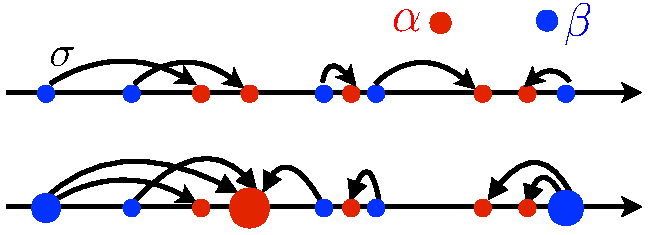
\includegraphics[width=.65\linewidth]{1d-discrete/1d-schematic}
\caption{\label{fig-1d-discrete}
1-D optimal couplings: each arrow $x_i \rightarrow y_j$ indicates a nonzero $\P_{i,j}$ in the optimal coupling.
%
Top: empirical measures with same number of points (optimal matching).
Bottom: generic case.
%
This corresponds to monotone rearrangements, if $x_i \leq x_{i'}$ are such that $\P_{i,j} \neq 0, \P_{i',j'} \neq 0$, then necessarily $y_j \leq y_{j'}$.
}
\end{figure}


% \bar x_{\si_1(i)} --> \bar y_{\si_2(i)}  k --> \si_2(\si_1^{-1}(k))
%%%%%%%
\begin{rem1}{Histogram equalization}
One-dimensional op\-ti\-mal tr\-ans\-port can be used to perform histogram equalization, with applications to the normalization of the palette of grayscale images, see Figure~\ref{fig-hist-eq}. In this case, one denotes $(\bar x_i)_i$ and $(\bar y_j)_j$ the gray color levels ($0$ for black, $1$ for white, and all values in between) of all pixels of the two input images enumerated in a predefined order (\ie columnwise). Assuming the number of pixels in each image is the same and equal to $n\times m$, sorting these color levels defines $x_i = \bar x_{\si_1(i)}$ and $y_j = \bar y_{\si_2(j)}$ as in Remark~\ref{rem-1d-empir}, where $\si_1, \si_2 : \{1,\ldots,nm\} \rightarrow \{1,\ldots,nm\}$ are permutations, so that $\si \eqdef \si_2 \circ \si_1^{-1}$ is the optimal assignment between the two discrete distributions. For image processing applications, $(\bar y_{\si(i)})_i$ defines the color values of an equalized version of $\bar x$, whose empirical distribution matches exactly the one of $\bar y$. The equalized version of that image can be recovered by folding back that $nm$-dimensional vector as an image of size $n\times m$. Also, $t \in [0,1] \mapsto (1-t) \bar x_{i} + t \bar y_{\si(i)}$ defines an interpolation between the original image and the equalized one, whose empirical distribution of pixels is the displacement interpolation (as defined in~\eqref{eq-displacement-1d-cumul}) between those of the inputs.
\end{rem1}
%%%%%%%

\begin{figure}[h!]
\centering
\begin{tabular}{@{}c@{\hspace{1mm}}c@{\hspace{1mm}}c@{\hspace{1mm}}c@{\hspace{1mm}}c@{\hspace{1mm}}@{}}
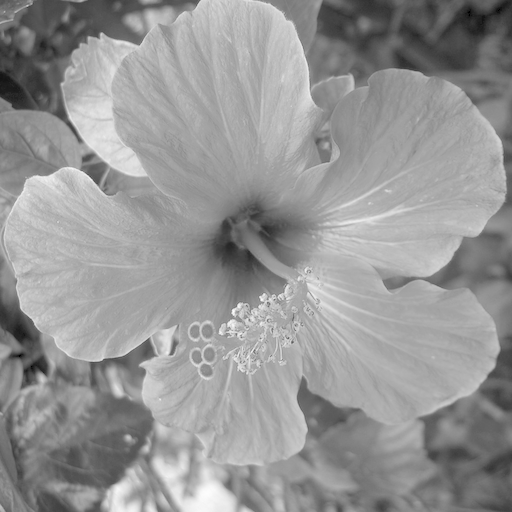
\includegraphics[width=.19\linewidth]{hist-eq/equalized-1}&
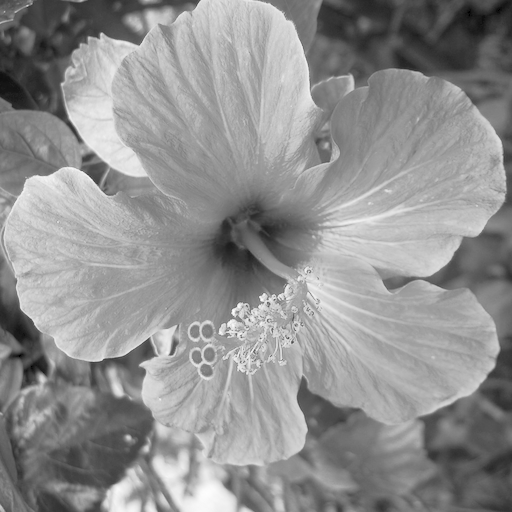
\includegraphics[width=.19\linewidth]{hist-eq/equalized-3}&
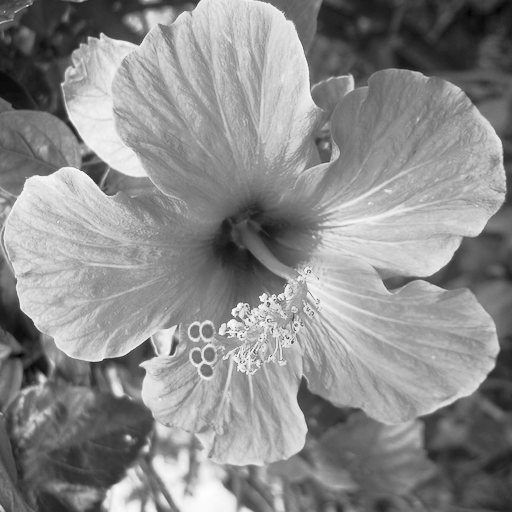
\includegraphics[width=.19\linewidth]{hist-eq/equalized-5}&
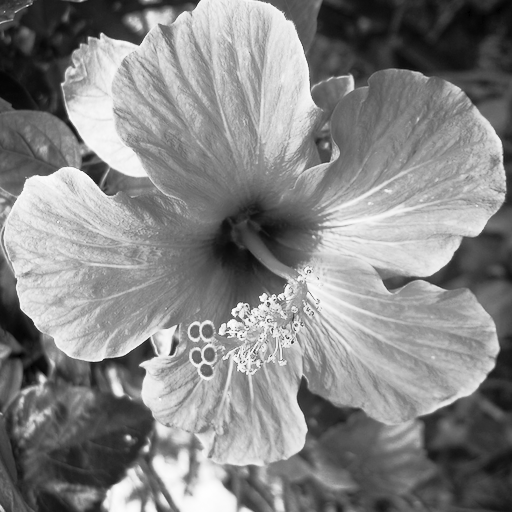
\includegraphics[width=.19\linewidth]{hist-eq/equalized-7}&
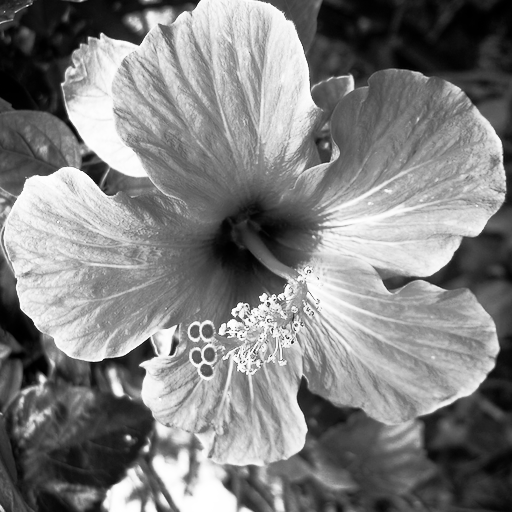
\includegraphics[width=.19\linewidth]{hist-eq/equalized-9}\\
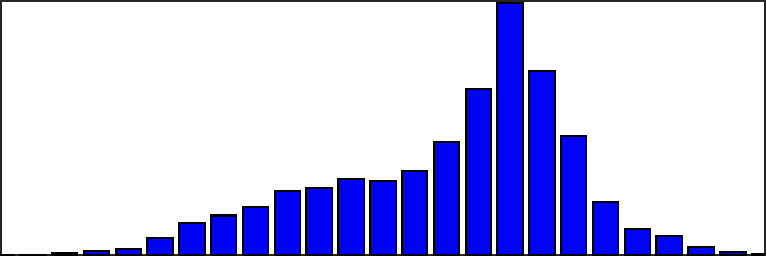
\includegraphics[width=.19\linewidth]{hist-eq/equalize-1}&
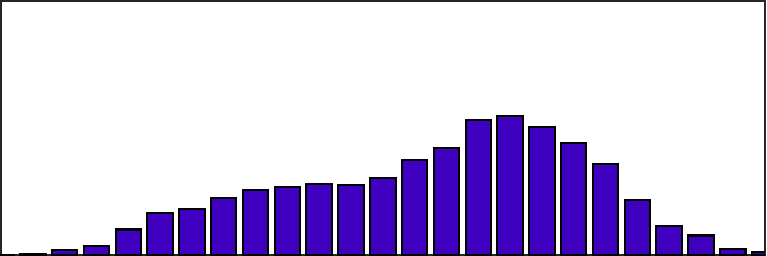
\includegraphics[width=.19\linewidth]{hist-eq/equalize-3}&
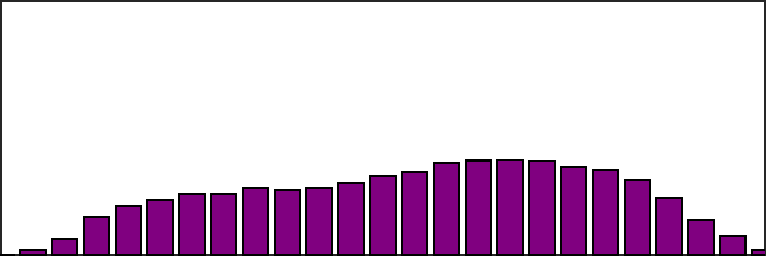
\includegraphics[width=.19\linewidth]{hist-eq/equalize-5}&
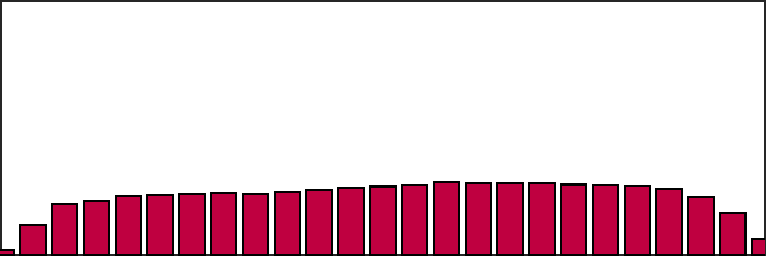
\includegraphics[width=.19\linewidth]{hist-eq/equalize-7}&
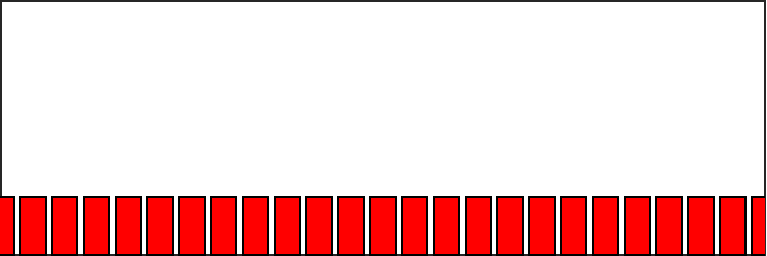
\includegraphics[width=.19\linewidth]{hist-eq/equalize-9}\\
$t=0$ & $t=0.25$& $t=0.5$& $t=.75$& $t=1$
\end{tabular}
\caption{\label{fig-hist-eq}
Histogram equalization for image processing, where $t$ parameterizes the displacement interpolation between the histograms.
}
\end{figure}


%%%%%%%
\begin{rem2}{1-D case---Generic case}\label{rem-1d-ot-generic}
For a measure $\al$ on $\RR$, we introduce the cumulative distribution function from $\RR$ to $\rightarrow [0,1]$ defined as
\eql{\label{eq-cumul-defn}
	\foralls x \in \RR, \quad \cumul{\al}(x) \eqdef \int_{-\infty}^x \d\al,
}
and its pseudoinverse  $\cumul{\al}^{-1} : [0,1] \rightarrow \RR \cup \{-\infty\}$
\eql{\label{eq-pseudo-inv-cum}
	\foralls r \in [0,1], \quad \cumul{\al}^{-1}(r) = \umin{x} \enscond{x \in \RR \cup \{-\infty\} }{ \cumul{\al}(x) \geq r }.
}
%
That function is also called the generalized quantile function of $\alpha$. For any $p \geq 1$, one has
\eql{\label{eq-wass-cumul}
	\Wass_p(\al,\be)^p = \norm{ \cumul{\al}^{-1} - \cumul{\be}^{-1} }_{L^p([0,1])}^p = \int_0^1 | \cumul{\al}^{-1}(r) - \cumul{\be}^{-1}(r) |^p \d r.
}
This means that through the map $\al \mapsto \cumul{\al}^{-1}$, the Wasserstein distance is isometric to a linear space equipped with the $L^p$ norm or, equivalently, that the Wasserstein distance for measures on the real line is a Hilbertian metric.
This makes the geometry of 1-D optimal transport very simple but also very different from its geometry in higher dimensions, which is not Hilbertian as discussed in Proposition~\ref{prop-negative-definite} and more generally in~\S\ref{sec-non-embeddability}.
%
For $p=1$, one even has the simpler formula
\begin{align}\label{eq-w1-1d}
	\Wass_1(\al,\be) &= \norm{ \cumul{\al} - \cumul{\be} }_{L^1(\RR)} =
	\int_\RR | \cumul{\al}(x) - \cumul{\be}(x) | \d x \\
	&= \int_\RR \abs{ \int_{-\infty}^x \d(\al-\be) } \d x,
\end{align}
which shows that $\Wass_1$ is a norm (see~\S\ref{sec-w1-eucl} for the generalization to arbitrary dimensions).
%
An optimal Monge map $\T$ such that $\T_\sharp \al=\be$ is then defined by
\eql{\label{eq-OT-map-1d}
 	\T = \cumul{\be}^{-1} \circ \cumul{\al}.
}
Figure~\ref{fig-1d-ot} illustrates the computation of 1-D OT through cumulative functions. It also displays displacement interpolations, computed as detailed in~\eqref{eq-displacement-1d-cumul}; see also Remark~\ref{rem-bary-1d}. For a detailed survey of the properties of optimal transport in one dimension, we refer the reader to~\cite[Chapter 2]{SantambrogioBook}.
\end{rem2}
%%%%%%%


\newcommand{\MyFigCumulMeas}[1]{\includegraphics[width=.33\linewidth]{1d-cumulative/#1}}
\newcommand{\MyFigCumulCum}[1]{\includegraphics[width=.24\linewidth]{1d-cumulative/#1}}
\begin{figure}[ht!]
\centering
\begin{tabular}{@{}c@{\hspace{1mm}}c@{\hspace{1mm}}c@{}}
\MyFigCumulMeas{input-mu}&
\MyFigCumulMeas{input-nu}&
\MyFigCumulMeas{interp-bary}\\
$\mu$ & $\nu$ & ${ (t\T+(1-t)\Id)_\sharp \mu}$
\end{tabular}
%%%%
\begin{tabular}{@{}c@{\hspace{2mm}}c@{\hspace{2mm}}c@{\hspace{2mm}}c@{}}
\MyFigCumulCum{cumul}&
\MyFigCumulCum{icumul}&
\MyFigCumulCum{transports}&
\MyFigCumulCum{interp-cumul}\\
$(\cumul{\al},\cumul{\be})$ &
$(\cumul{\al}^{-1},\cumul{\be}^{-1})$ &
$(T,T^{-1})$ &
$(1-t)\cumul{\al}^{-1}+t\cumul{\be}^{-1}$
\end{tabular}
\caption{\label{fig-1d-ot}
Computation of OT and displacement interpolation between two 1-D measures, using cumulant function as detailed in~\eqref{eq-OT-map-1d}.
}
\end{figure}

%%%%%%%
\begin{rem2}{Distance between Gaussians}\label{rem-dist-gaussians}
If $\al = \Nn(\mean_\al,\cov_\al)$ and $\be = \Nn(\mean_\be,\cov_\be)$ are two Gaussians in $\RR^\dim$, then one can show that the following map
\eql{\label{eq-transport-Bures}T:x\mapsto \mean_\be + A(x-\mean_\al),}
where
$$A=\cov_\al^{-\tfrac{1}{2}}\Big(\cov_\al^{\tfrac{1}{2}}\cov_\be\cov_\al^{\tfrac{1}{2}}\Big)^{\tfrac{1}{2}}\cov_\al^{-\tfrac{1}{2}}=\transp{A},$$
is such that $T_\sharp \rho_\al = \rho_\be$. Indeed, one simply has to notice that the change of variables formula~\eqref{eq-pfwd-density} is satisfied since
$$
\begin{aligned}\rho_\be(T(x))&=\det(2\pi\cov_\be)^{-\tfrac{1}{2}} \exp(-\dotp{T(x)-\mean_\be}{\cov_\be^{-1}(T(x)-\mean_\be)})\\
&= \det(2\pi\cov_\be)^{-\tfrac{1}{2}} \exp(-\dotp{ x-\mean_\al}{\transp{A}\cov_\be^{-1}A(x-\mean_\al)}) \\
&= \det(2\pi\cov_\be)^{-\tfrac{1}{2}} \exp(-\dotp{ x-\mean_\al}{\cov_\al^{-1}(x-\mean_\al)}),
\end{aligned}$$
and since $T$ is a linear map we have that
$$|\det T'(x)|= \det A = \left(\frac{\det\cov_\be}{\det\cov_\al}\right)^{\tfrac{1}{2}}$$
 and we therefore recover $\rho_\al=|\det T'| \rho_\be$ meaning $T_\sharp \al = \be$. Notice now that $T$ is the gradient of the convex function $\psi:x\mapsto \tfrac{1}{2}\dotp{x-\mean_\al}{A (x-\mean_\al)} + \dotp{\mean_\be}{x}$ to conclude, using~\citeauthor{Brenier91}'s theorem~\citeyearpar{Brenier91} (see Remark~\ref{rem-exist-mongemap}), that $T$ is optimal. Both that map $T$ and the corresponding potential $\psi$ are illustrated in Figures~\ref{fig-gaussians-2d-T} and~\ref{fig-gaussians-2d-psi}

With additional calculations involving first and second order moments of $\rho_\al$, we obtain that the transport cost of that map is
\eql{\label{eq-dist-gauss}
	\Wass_2^2( \al,\be ) = \norm{ \mean_\al - \mean_\be }^2 + \Bb(\cov_\al,\cov_\be)^2,
}
where $\Bb$ is the so-called~\citeauthor{bures1969extension} metric~\citeyearpar{bures1969extension} between positive definite matrices (see also~\citet{,forrester2016relating}),
\eql{\label{eq-bure-defn}
	\Bb(\cov_\al,\cov_\be)^2 \eqdef \tr\pa{
		\cov_\al + \cov_\be - 2 ( \cov_\al^{1/2} \cov_\be \cov_\al^{1/2} )^{1/2}
	},
}
where $\cov^{1/2}$ is the matrix square root. One can show that $\Bb$ is a distance on covariance matrices and that $\Bb^2$ is convex with respect to both its arguments. \todoK{ref ? proof ? }
In the case where $\cov_\al = \diag(r_i)_i$ and $\cov_\be = \diag(s_i)_i$ are diagonals, the Bures metric is the Hellinger distance
\eq{
	\Bb(\cov_\al,\cov_\be) = \norm{ \sqrt{r}-\sqrt{s} }_2.
}
For 1-D Gaussians, $\Wass_2$ is thus the Euclidean distance on the 2-D plane plotting the mean and the standard deviation of a Gaussian $(\mean,\sqrt{\cov})$, as illustrated in Figure~\ref{fig-1d-gaussian}.
%
For a detailed treatment of the Wasserstein geometry of Gaussian distributions, we refer to~\citet{takatsu2011wasserstein}, and for additional considerations on the Bures metric the reader can consult the very recent references~\citep{malago2018wasserstein,bhatia2018bures}. One can also consult~\citep{NIPS2018_8226} for a a recent application of this metric to compute probabilistic embeddings for words,~\citep{NIPS2018_8067} to see how it is used to compute a robust extension to Kalman filtering, or~\citep{NIPS2017_7149} in which it is applied to covariance functions in reproducing kernel Hilbert spaces.
\end{rem2}
%%%%%%
\begin{figure}[h!]
\centering
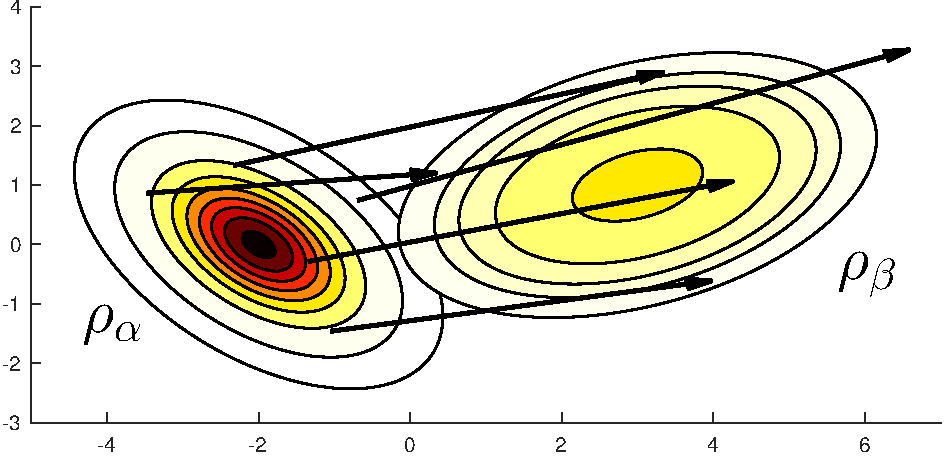
\includegraphics[width=.7\linewidth]{gaussians-2d/gaussians1.pdf}
\caption{\label{fig-gaussians-2d-T} Two Gaussians $\rho_\al$ and $\rho_\be$, represented using the contour plots of their densities, with respective mean and variance matrices $\mean_\al=(-2,0),\cov_\al=\frac{1}{2}\left(1 -\tfrac{1}{2};-\tfrac{1}{2}  1\right)$ and $\mean_\be=(3,1), \cov_\be=\left(2, \tfrac{1}{2}; \tfrac{1}{2}, 1\right)$. The arrows originate at random points $x$ taken on the plane and end at the corresponding mappings of those points $T(x)=\mean_\be + A(x-\mean_\al)$.}
\end{figure}



%%%%%%%
\begin{rem2}{Distance between elliptically contoured distributions}\label{rem-dist-elliptic}
\citeauthor{gelbrich1990formula} provides a more general result than that provided in Remark~\ref{rem-dist-gaussians}: the Bures metric between Gaussians extends more generally to \emph{elliptically contoured distributions}~\citeyearpar{gelbrich1990formula}.
%
In a nutshell, one can first show that for two measures with given mean and covariance matrices, the distance between the two Gaussians with these respective parameters is a lower bound of the Wasserstein distance between the two measures~\citep[Theorem 2.1]{gelbrich1990formula}. Additionally, the closed form~\eqref{eq-dist-gauss} extends to families of elliptically contoured densities: If two densities $\rho_\al$ and $\rho_\be$ belong to such a family, namely when $\rho_\al$ and $\rho_\be$ can be written for any point $x$ using a mean and positive definite parameter,

\eq{\begin{aligned}\rho_\al(x) = \frac{1}{\sqrt{\det(\A)}}h(\dotp{x-\mean_\al}{\A^{-1}(x-\mean_\al)})\\ \rho_\be(x)= \frac{1}{\sqrt{\det(\B)}} h(\dotp{x-\mean_\be}{\B^{-1}(x-\mean_\be)}),\end{aligned}}
for the same nonnegative valued function $h$ such that the integral $$\int_{\RR^\dim} h(\dotp{x}{x})dx=1,$$ then their optimal transport map is also the linear map \eqref{eq-transport-Bures} and their Wasserstein distance is also given by the expression $\eqref{eq-dist-gauss}$, with a slightly different scaling of the Bures metric that depends only the generator function $h$. For instance, that scaling is $1$ for Gaussians ($h(t)=e^{-t/2}$) and $1/(\dim+2)$ for uniform distributions on ellipsoids ($h$ the indicator function for $[0,1]$). This result follows from the fact that the covariance matrix of an elliptic distribution is a constant times its positive definite parameter~\citep[Theo. 4(ii)]{gomez2003survey} and that the Wasserstein distance between elliptic distributions is a function of the Bures distance between their covariance matrices~\citep[Cor. 2.5]{gelbrich1990formula}.
\end{rem2}
%%%%%%
\begin{figure}[h!]
\centering
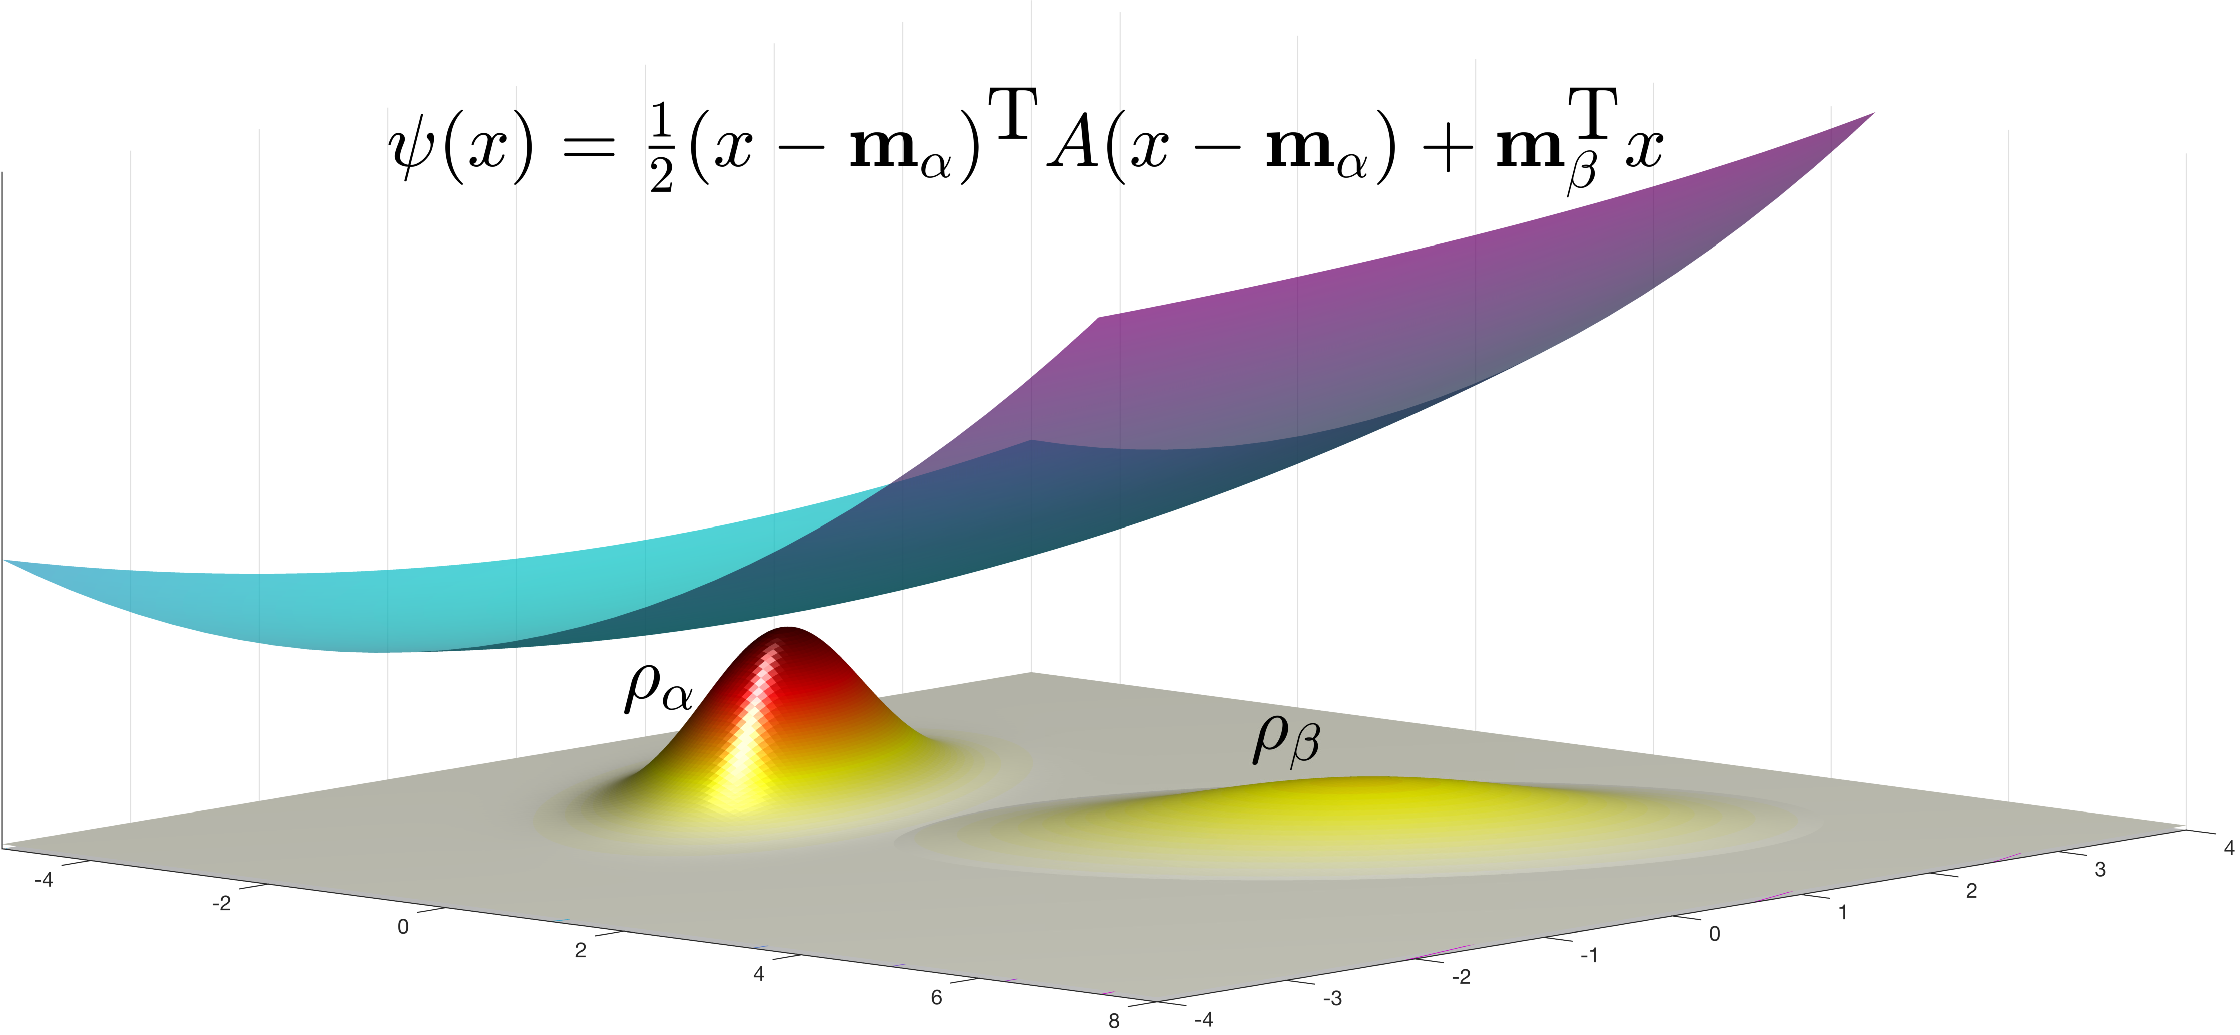
\includegraphics[width=.85\linewidth]{gaussians-2d/gaussians2.pdf}
\caption{\protect\label{fig-gaussians-2d-psi} Same Gaussians $\rho_\al$ and $\rho_\be$ as defined in Figure~\ref{fig-gaussians-2d-T}, represented this time as surfaces. The surface above is the Brenier potential $\psi$ defined up to an additive constant (here +50) such that $T=\nabla \psi$. For visual purposes, both Gaussian densities have been multiplied by a factor of 100.}
\end{figure}

\begin{figure}[h!]
\centering
\begin{tabular}{@{}c@{\hspace{1mm}}c@{}}
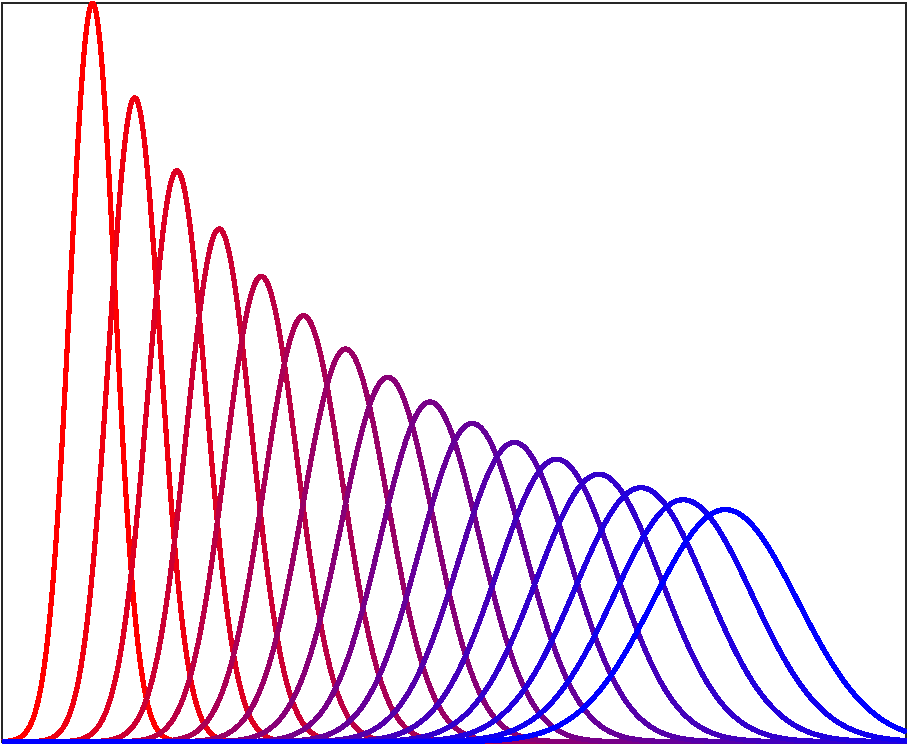
\includegraphics[width=.35\linewidth]{gaussian-1d/interp-density}
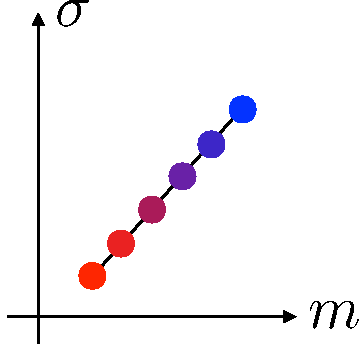
\includegraphics[width=.25\linewidth]{gaussian-1d/gaussian-param}
\end{tabular}
\caption{\label{fig-1d-gaussian}
Computation of displacement interpolation between two 1-D Gaussians.
%
Denoting $\Gg_{m,\si}(x) \eqdef \frac{1}{\sqrt{2\pi}s}e^{-\frac{(x-m)^2}{2s^2}}$ the Gaussian density, it thus shows
the interpolation $\Gg_{(1-t)m_0+t m_1,(1-t)\si_0+t \si_1}$.
}
\end{figure}



\todoK{Maybe cover the case of translation / scaling of the same input. Explain that $\Wass$ is invariant to isometries. }
